% !TEX TS-program = pdflatex
% !TEX encoding = UTF-8 Unicode

%\documentclass[ing,male,java,dept460,oneside]{diploma}
\documentclass{article}

\usepackage[czech]{babel}
\usepackage[T1]{fontenc}
\usepackage[utf8]{inputenc}
\usepackage{color}
\usepackage{geometry}
\usepackage{float}
\usepackage{graphicx}
\usepackage[stable]{footmisc}
\usepackage{hyperref}
\usepackage{amsfonts}
 \usepackage{bbm}
 \usepackage{booktabs}
 \usepackage{url}
 \usepackage{nameref}
 \usepackage{caption}
 \usepackage{subcaption}
 \usepackage{listings}



% \ThesisAuthor{Josef Raška}

% U bakalarske praxe neni nutne nazev zadavat
%\ThesisTitle{Tos ten android ze}

% U bakalarske prace neni nutne anglicky nazev zadavat
%\EnglishThesisTitle{The Android stuff}

%\SubmissionDate{29. dubna 2016}

%\PrintPublicationAgreement{true}


%\Thanks{Podekovani \newline Dalsi lajna }


%\CzechAbstract{Cesky abstrakt}

%\CzechKeywords{vlastní číslo, vlastní vektor, vlastní dvojice, aplikace vlastních čísel, mocninná metoda, Lanczosova metoda, předpodmínění}

%\EnglishAbstract{English abstract}

%\EnglishKeywords{Android, development}

\renewcommand{\lstlistingname}{Ukázka kódu}
\renewcommand{\lstlistlistingname}{List of ukázek kódu s}

\usepackage{inconsolata}
\lstset{ %
%  backgroundcolor=\color{white},   % choose the background color; you must add \usepackage{color} or \usepackage{xcolor}
  basicstyle=\footnotesize,        % the size of the fonts that are used for the code
%  breakatwhitespace=false,         % sets if automatic breaks should only happen at whitespace
%  breaklines=true,                 % sets automatic line breaking
  captionpos=b,                    % sets the caption-position to bottom
%  commentstyle=\color{mygreen},    % comment style
%  deletekeywords={...},            % if you want to delete keywords from the given language
%  escapeinside={\%*}{*)},          % if you want to add LaTeX within your code
%  extendedchars=true,              % lets you use non-ASCII characters; for 8-bits encodings only, does not work with UTF-8
  frame=single,	                   % adds a frame around the code
  keepspaces=true,                 % keeps spaces in text, useful for keeping indentation of code (possibly needs columns=flexible)
  keywordstyle=\color{blue},       % keyword style
  language=Java,                 % the language of the code
%  otherkeywords={*,...},           % if you want to add more keywords to the set
 inputencoding=utf8,
  numbers=none,                    % where to put the line-numbers; possible values are (none, left, right)
%  numbersep=5pt,                   % how far the line-numbers are from the code
%  numberstyle=\tiny\color{mygray}, % the style that is used for the line-numbers
  rulecolor=\color{black},         % if not set, the frame-color may be changed on line-breaks within not-black text (e.g. comments (green here))
%  showspaces=false,                % show spaces everywhere adding particular underscores; it overrides 'showstringspaces'
%  showstringspaces=false,          % underline spaces within strings only
  showtabs=false,                  % show tabs within strings adding particular underscores
%  stepnumber=2,                    % the step between two line-numbers. If it's 1, each line will be numbered
%  stringstyle=\color{mymauve},     % string literal style
  tabsize=2,	                   % sets default tabsize to 2 spaces
  literate={á}{{\'a}}1 {é}{{\'e}}1  {č}{{\'c}}1 {ý}{{\'y}}1 {í}{{\'i}}1 {ú}{{\'u}}1,
%  title=\lstname                   % show the filename of files included with \lstinputlisting; also try caption instead of title
}

\title{Diplomová práce}
\author{Josef Raška \(ras0029\)}
\newtheorem{priklad}{Příklad}[section]
\newtheorem{veta}{Věta}[section]
\newtheorem{alg}{Algoritmus}[section]

\newcommand{\usecase}[2]{\subsubsection{#1}\label{#2}}
\setcounter{tocdepth}{2}

\begin{document}
%\maketitle
%\MakeTitlePages
\urlstyle{same}

\tableofcontents
\listoffigures
\listoftables
%\lstlistoflistings

\newpage

\section{Úvod}

\section{Návrh aplikace}
\subsection{Popis aktérů}
\begin{figure}[H]
        \centering
                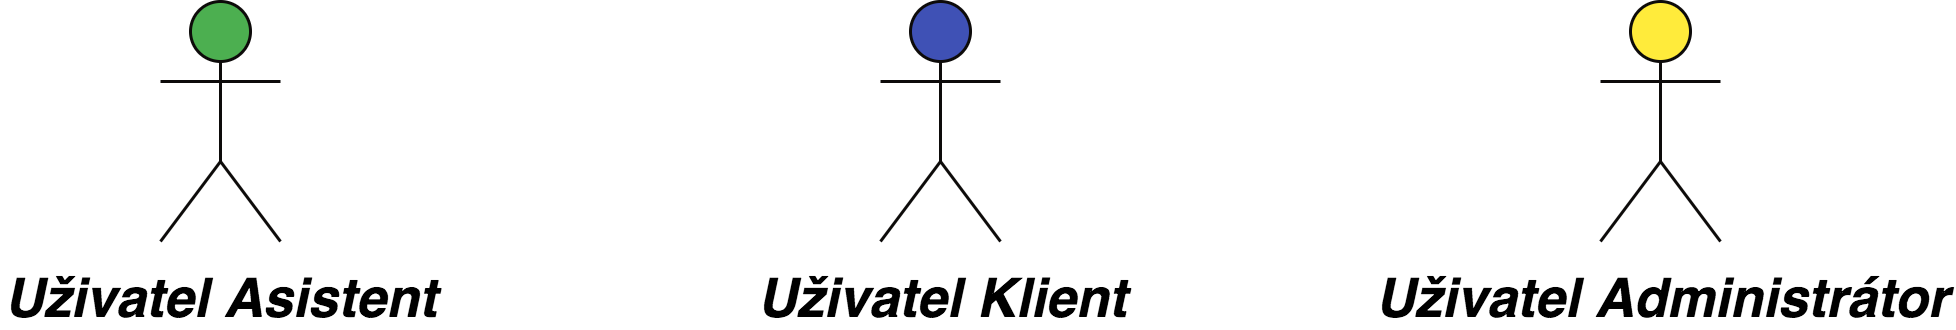
\includegraphics[scale=0.14]{img/actors.png}
        \caption{Aktéři systému}
        \label{fig:actors}
\end{figure}

Pro uživatele klienta i asistenta jsou definovány případy užití zvlášť, neboť se celé chování
a použití aplikace bude v obou případech značně lišit. Grafické zobrazní aktéru je na obrázku~\ref{fig:actors}.

\subsubsection{Uživatel Asistent}
Jedná se o aktéra, který je zároveň klientovi s mentálním postižením odborným asistentem,
jenž o něj pečuje a poskytuje mu podporu. Tento aktér je relevantní k vytváření obsahu,
který má pomoci klientovi k lepší orientaci při cestování a také mu může připravenou
cestu předvést. Může také nahraná data editovat a případně je rozšiřovat. Může také zadat
do aplikace zadat své kontaktní údaje pro možnou nečekanou situaci klienta na cestách, případně
nastavit zálohování uložených dat pro zamezení jejich ztráty při ztrátě telefonu nebo jeho výměně
za jiný.

\subsubsection{Uživatel Klient}
Klient je osoba pro kterou je aplikace primárně určena a má mu pomoci vyřešit problém,
v tomto případě pomoci z orientací při cestování. Může si prohlížet obsah a zejména ho
využívat při cestách v terénu. Uživatel by měl být upozorněn na všechny uložené a rozeznané
data v závislosti na své pozici a měl by tak získat relevantní informace k tomu, kde se právě
nachází. Dále může aplikaci využít ke snadnému kontaktování svého asistenta.



\subsubsection{Uživatel Administrátor}


\subsection{Use casy uživatel Asistent}
Pro uživatele asistenta jsou určeny složitější operace pro vytváření interaktivního obsahu pro klienta,
nastavování aplikace a prezentace klientovi. Pro use casy asistenta platí, že klient může těmto
krokům přihlížet, pokud o to projeví zájem. Use casy asistenta a jejich vztahy lze vidět na obrázku~\ref{fig:UseCasesAsistant}.

\begin{figure}[H]
        \centering
                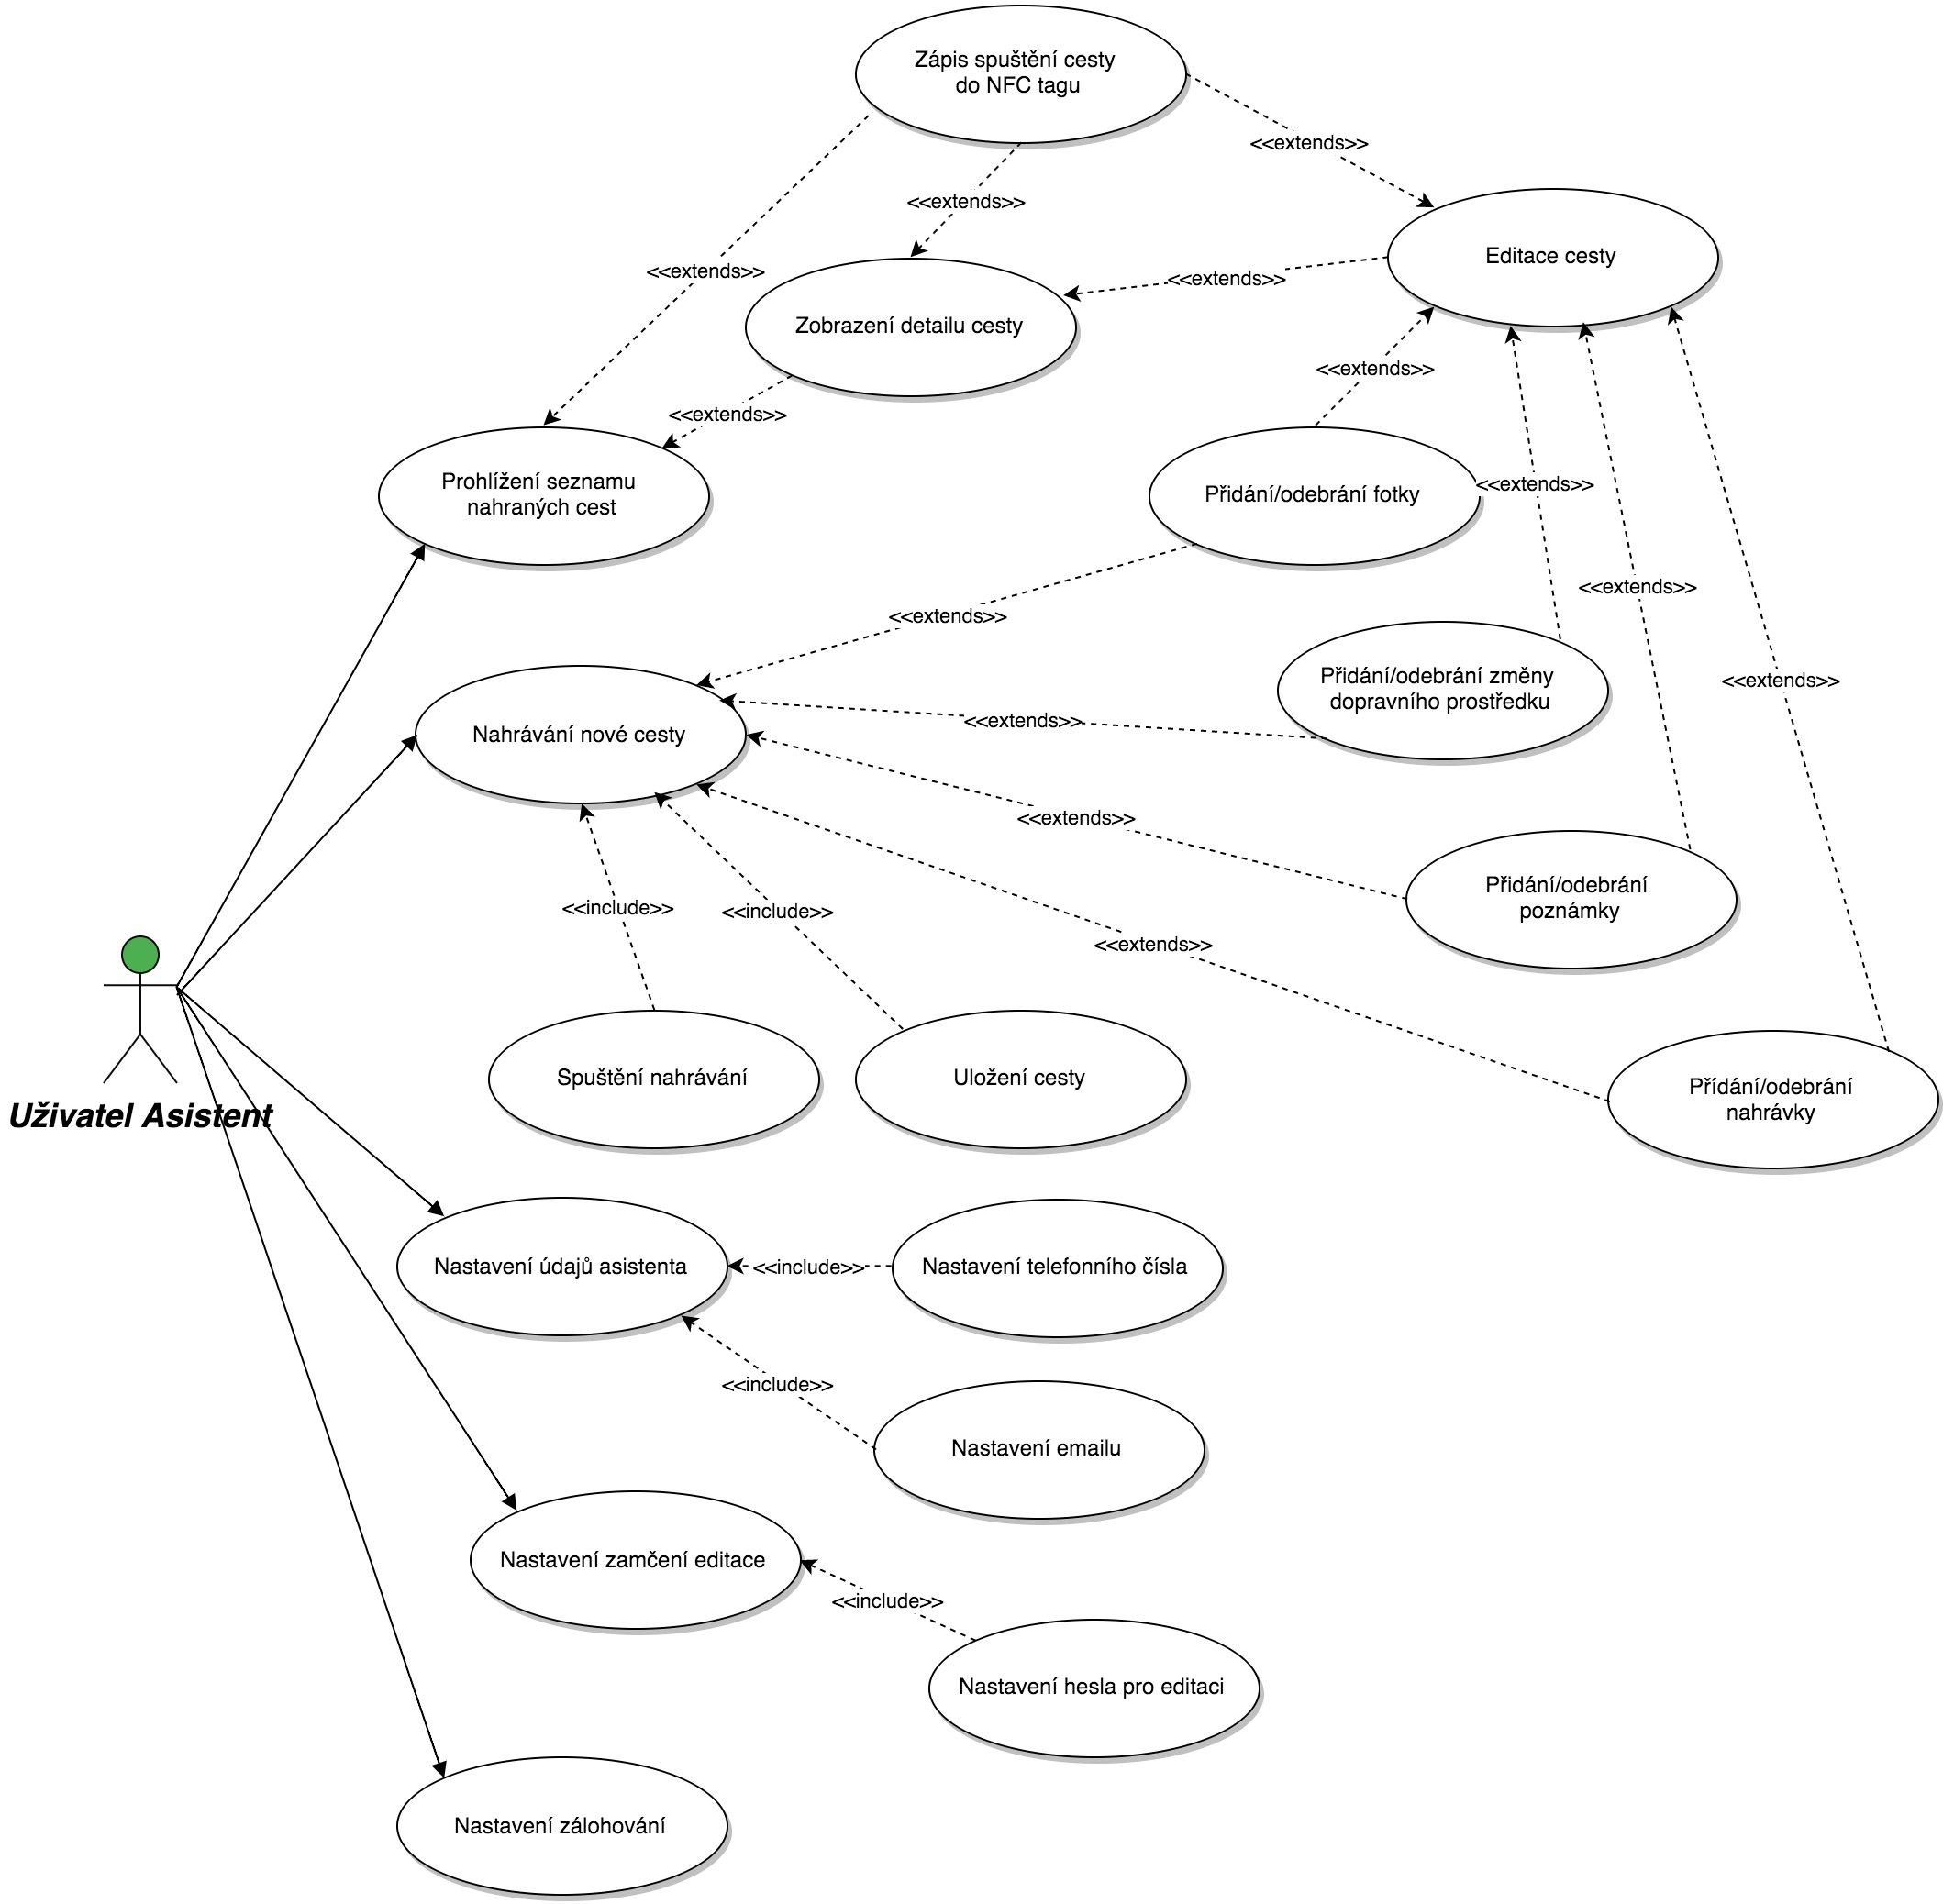
\includegraphics[scale=0.2]{img/UseCasesAsistant.png}
        \caption{Diagram use casů uživatele asistent}
        \label{fig:UseCasesAsistant}
\end{figure}

\usecase{Prohlížení seznamu nahraných cest}{prohlizeniasistent}
\textbf{Aktéři:} Asistent

\vspace{0.1cm}
\noindent
\textbf{Hlavní scénář:} Na úvodní obrazovce jsou zobrazeny všechny dosud nahrané cesty ve seznamu pod sebou.
Lze vidět pouze základní údaje a přiřazený obrázek pro snadnou orientaci. Uživatel se pomocí
kliknutí na řádek může podívat na celý detail cesty, případně pomocí rychlých akcí spustit ihned asistenci
a podobně. Obrazovku prohlížení cest lze vidět na obrázku~\ref{fig:prohlizeniasistent}.

\vspace{0.1cm}
\noindent
\textbf{Spouštěč:} Uživatel spustí aplikaci nebo se do ní vrátí pomocí notifikace v notifikační liště.

\vspace{0.1cm}
\noindent
\textbf{Rozšíření:}
\begin{itemize}
  \item \nameref{nahravanicesty}
  \item \nameref{detailasistent}
  \item \nameref{nfczapis}
\end{itemize}

\begin{figure}[H]
\begin{minipage}{.5\textwidth}
\centering
                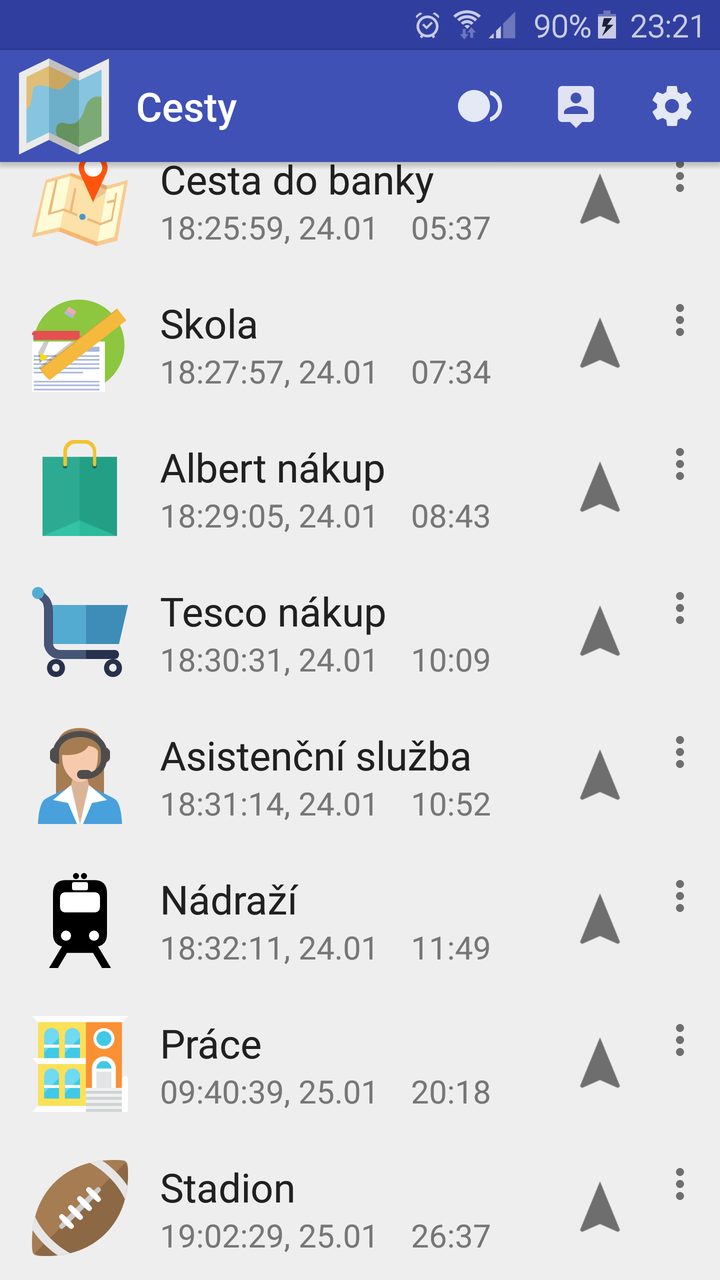
\includegraphics[scale=0.14]{img/screen/seznamcest.png}
        \caption{Prohlížení seznamu cest}
        \label{fig:prohlizeniasistent}
\end{minipage}
\begin{minipage}{.5\textwidth}
    \centering
                    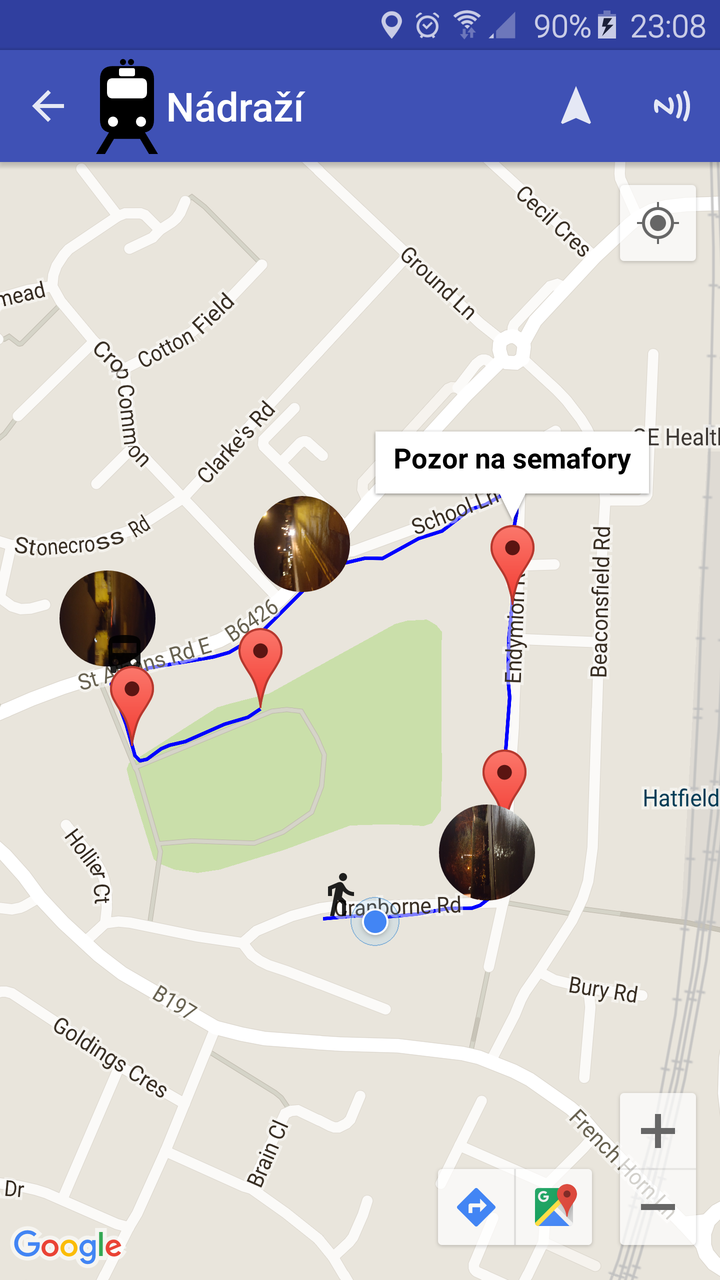
\includegraphics[scale=0.14]{img/screen/detailcesty.png}
            \caption{Zobrazení detailu cesty}
            \label{fig:detailasistent}

       \end{minipage}
\end{figure}

\usecase{Zobrazení detailu cesty}{detailasistent}
\textbf{Aktéři:} Asistent

\vspace{0.1cm}
\noindent
\textbf{Hlavní scénář:} Uživateli se zobrazí detail cesty se všemi informacemi, které jsou o ní uloženy.
Na mapě si může prohlédnout kudy vedla, an místech fotografií jsou miniatury fotek, při změně dopravních
prostředků lze vidět ikony daných prostředků, zvukově a textové záznamy jsou označeny příslušnou ikonou.
Při klepnutí na indikátor některého z těchto záznamů se zobrazí jeho popis, který uživatel dříve zadal.
V detailu cesty lze poklepáním na tlačítko editovat přejít do módu editace cesty a všechny dříve zmíněné
záznamy upravit. Ukázku lze vidět na obrázku~\ref{fig:detailasistent}.

\vspace{0.1cm}
\noindent
\textbf{Prekondice:} Cesta je uložena.

\vspace{0.1cm}
\noindent
\textbf{Spouštěč:} Uživatel klepne na řádek se zobrazenou cestou v seznamu cest.

\vspace{0.1cm}
\noindent
\textbf{Rozšíření:}
\begin{itemize}
  \item \nameref{editacecesty}
  \item \nameref{nfczapis}
\end{itemize}






\usecase{Zapsání cesty do NFC tagu}{nfczapis}
\textbf{Aktéři:} Asistent

\vspace{0.1cm}
\noindent
\textbf{Hlavní scénář:} Uživateli se zobrazí
obrazovka, která jej instruuje k přiložení NFC tagu k telefonu. Jakmile telefon zaznamená blízkost tagu,
zapíše do něj informaci o uložené cestě pro následné rychlé spouštění při přiložení tagu k telefonu.
Obrazovku zápisu do NFC tagu lze vidět na obrázku~\ref{fig:nfczapis} a oznámení o zapsaném tagu
na obrázku~\ref{fig:nfczapsano}.

\vspace{0.1cm}
\noindent
\textbf{Prekondice:} Cesta je uložena.

\vspace{0.1cm}
\noindent
\textbf{Spouštěč:} Uživatel klepne na ikonu NFC v detailu cesty nebo an rozšiřující menu v seznamu cest.


\begin{figure}[H]
\begin{minipage}{.5\textwidth}
\centering
                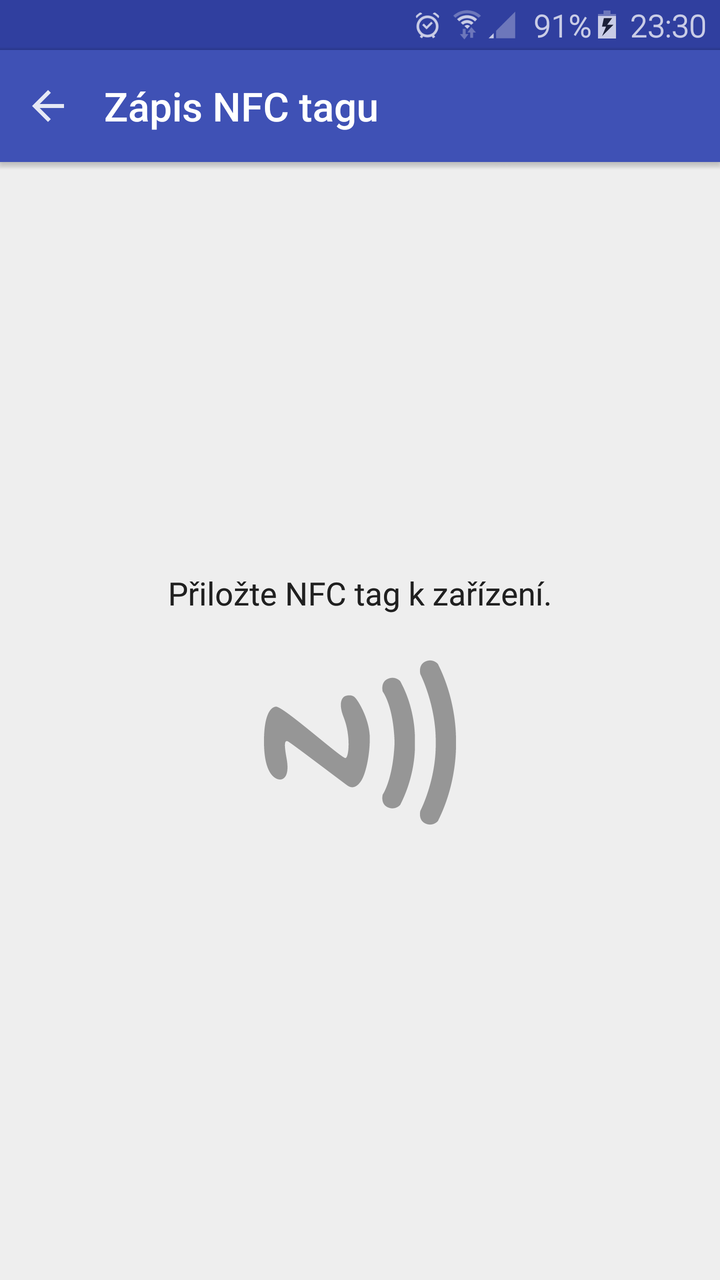
\includegraphics[scale=0.14]{img/screen/zapisnfcdetail.png}
        \caption{Zápis do NFC tagu}
        \label{fig:nfczapis}
\end{minipage}
\begin{minipage}{.5\textwidth}
    \centering
                    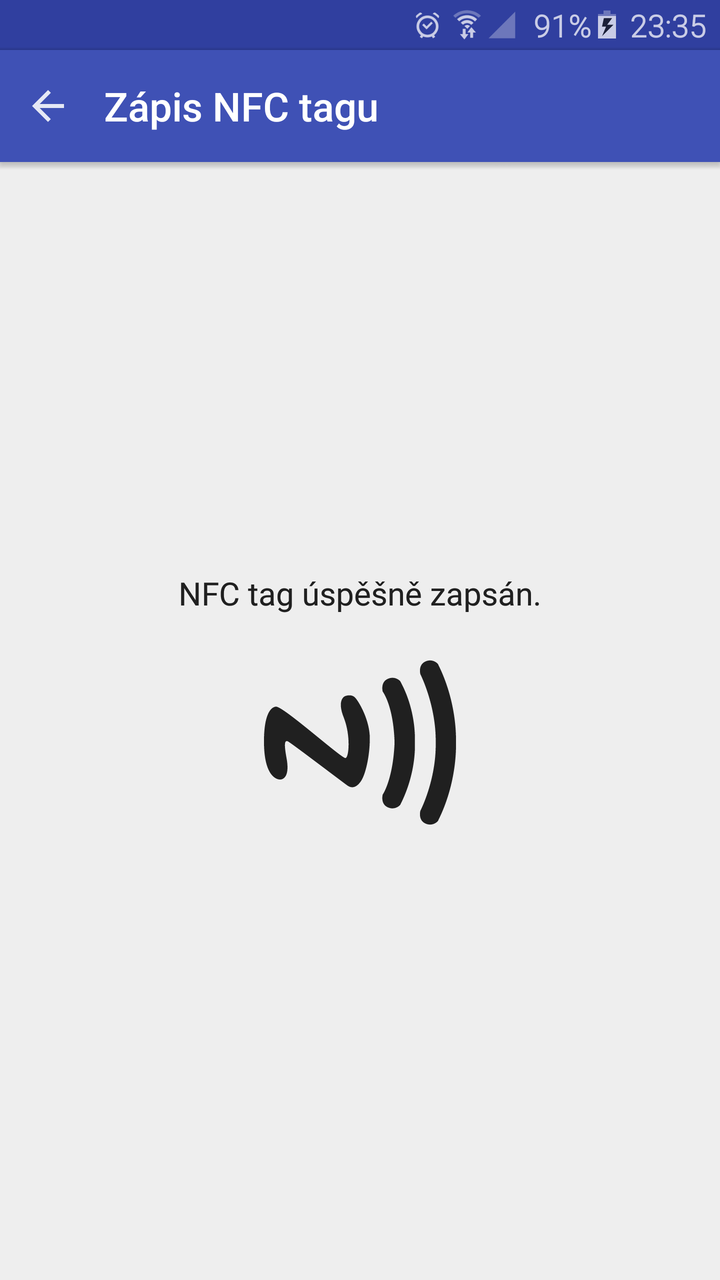
\includegraphics[scale=0.14]{img/screen/zapisdonfc.png}
            \caption{Zapsáno do NFC tagu}
            \label{fig:nfczapsano}

       \end{minipage}
\end{figure}



\usecase{Editace cesty}{editacecesty}
\textbf{Aktéři:} Asistent

\vspace{0.1cm}
\noindent
\textbf{Hlavní scénář:} Uživatel může editovat všechny uložené informace o cestě. Přepsání editačních
polí může změnit názvy a popis nahrané cesty, podržením a přetažením miniatur fotek nebo ikon dalších údajů na mapě může změnit
jejich pozici a tudíž místo, kdy se později vyvolají. Dále může podržením přetažením měnit tvar trasy,
při klepnutí na mapu přidat další záznamy. Jakmile je uživatel s editací spokojen, klepnutím na tlačítko
uložit se údaje zapíší do databáze a následující asistence cestování bude tyto údaje používat.

\vspace{0.1cm}
\noindent
\textbf{Prekondice:} Cesta je uložena.

\vspace{0.1cm}
\noindent
\textbf{Spouštěč:} Uživatel klepne na tlačítko editovat v detailu cesty.

\vspace{0.1cm}
\noindent
\textbf{Rozšíření:}
\begin{itemize}
  \item \nameref{pridanifotky}
  \item \nameref{pridaninahravky}
  \item \nameref{pridanipoznamky}
  \item \nameref{pridanizmenyprostredku}
    \item \nameref{odebranifotky}
    \item \nameref{odebraninahravky}
    \item \nameref{odebranipoznamky}
    \item \nameref{odebranizmenyprostredku}
\end{itemize}

\usecase{Přidání fotky}{pridanifotky}
\textbf{Aktéři:} Asistent

\vspace{0.1cm}
\noindent
\textbf{Hlavní scénář:} Spustí se fotoaparát zařízení a uživatel může začít fotit. Jakmile pořídí
fotografii, zobrazí se v aplikace okno pro zadání názvu fotky s dotazem pro uložení. Uživatel zadá název
a klepnutím na potvrzovací tlačítko se fotka uloží mezi data aplikace a zobrazí mezi aktuálními fotografiemi
na místě polohy uživatele v době pořízení fotografie. Uložení fotky lze vidět na obrázku~\ref{fig:pridanifotky}.

\vspace{0.1cm}
\noindent
\textbf{Prekondice:} Uživatel nahrává nebo edituje cestu.

\vspace{0.1cm}
\noindent
\textbf{Spouštěč:} Uživatel klepl na tlačítko přidat fotku.

\begin{figure}[H]
\begin{minipage}{.5\textwidth}
\centering
                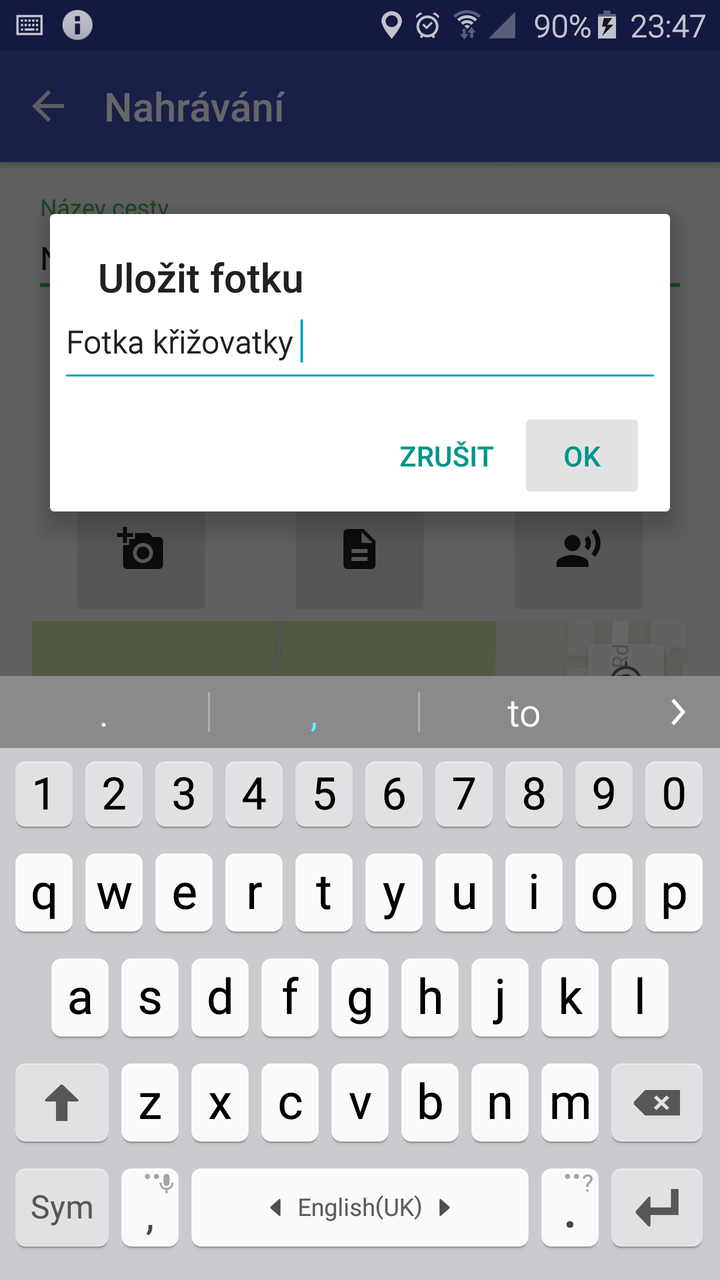
\includegraphics[scale=0.14]{img/screen/ulozenifotky.png}
        \caption{Pojmenování fotky po pořízení}
        \label{fig:pridanifotky}
\end{minipage}
\begin{minipage}{.5\textwidth}
     \centering
                     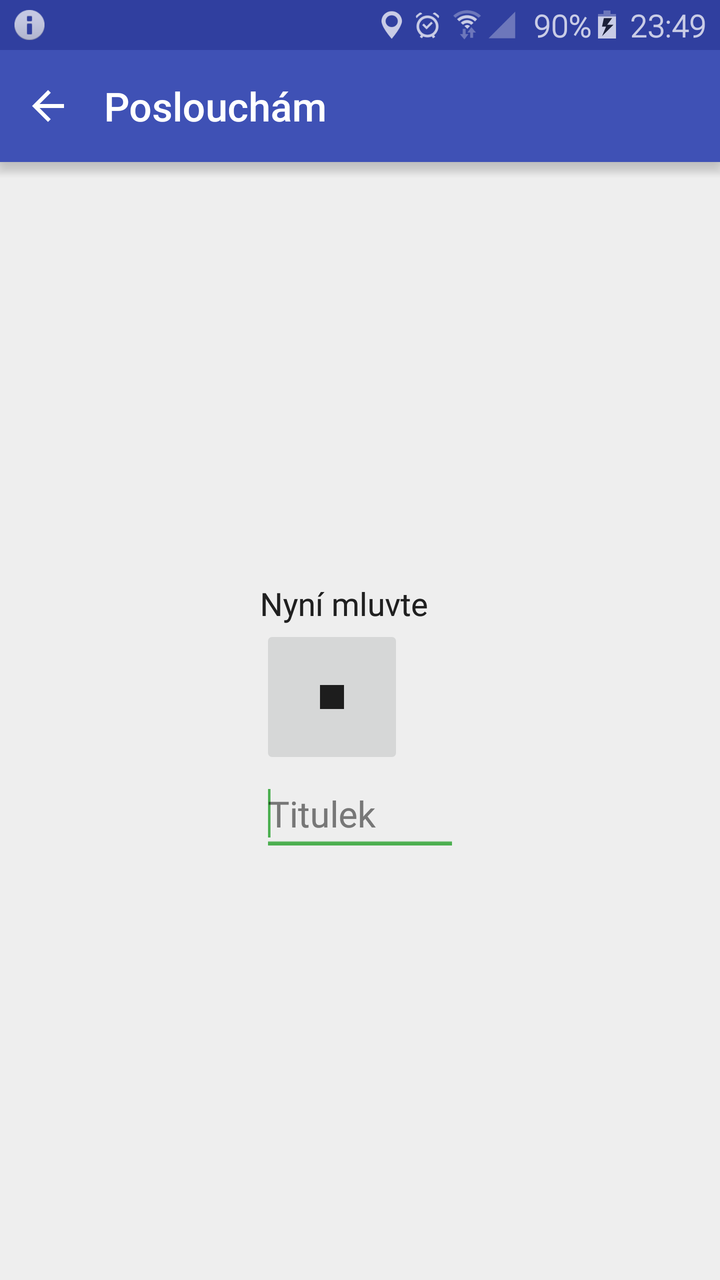
\includegraphics[scale=0.14]{img/screen/nahravaninahravky.png}
             \caption{Přidání zvukové nahrávky}
             \label{fig:pridaninahravky}

       \end{minipage}
\end{figure}

\usecase{Přidání zvukové nahrávky}{pridaninahravky}
\textbf{Aktéři:} Asistent

\vspace{0.1cm}
\noindent
\textbf{Hlavní scénář:} Uživateli se zobrazí obrazovka s textem mluvte a zvuk se zaznamenává.
Když je uživatel hotov, klepne na tlačítko stop a může nahrávce přidat název, který se bude později zobrazovat.
Poté tlačítkem nahrávku uloží mezi data aplikace s přiřazenou aktuální polohou uživatele.
Zobrazení nahrávání lze vidět na obrázku~\ref{fig:pridaninahravky}.

\vspace{0.1cm}
\noindent
\textbf{Prekondice:} Uživatel nahrává nebo edituje cestu.

\vspace{0.1cm}
\noindent
\textbf{Spouštěč:} Uživatel klepl na tlačítko přidat nahrávku.




\usecase{Přidání poznámky}{pridanipoznamky}
\textbf{Aktéři:} Asistent

\vspace{0.1cm}
\noindent
\textbf{Hlavní scénář:} Uživateli se zobrazí okno s textovým vstupem a vysune se klávesnice. Uživatel
zadá textovou poznámku a po klepnutí na potvrzovací tlačítko se poznámka uloží s asociací k aktuální poloze
uživatele. Okno přidávání poznámky lze vidět na obrázku~\ref{fig:pridanipoznamky}.

\vspace{0.1cm}
\noindent
\textbf{Prekondice:} Uživatel nahrává nebo edituje cestu.

\vspace{0.1cm}
\noindent
\textbf{Spouštěč:} Uživatel klepl na tlačítko přidat poznámku.

\begin{figure}[H]
\begin{minipage}{.5\textwidth}
\centering
                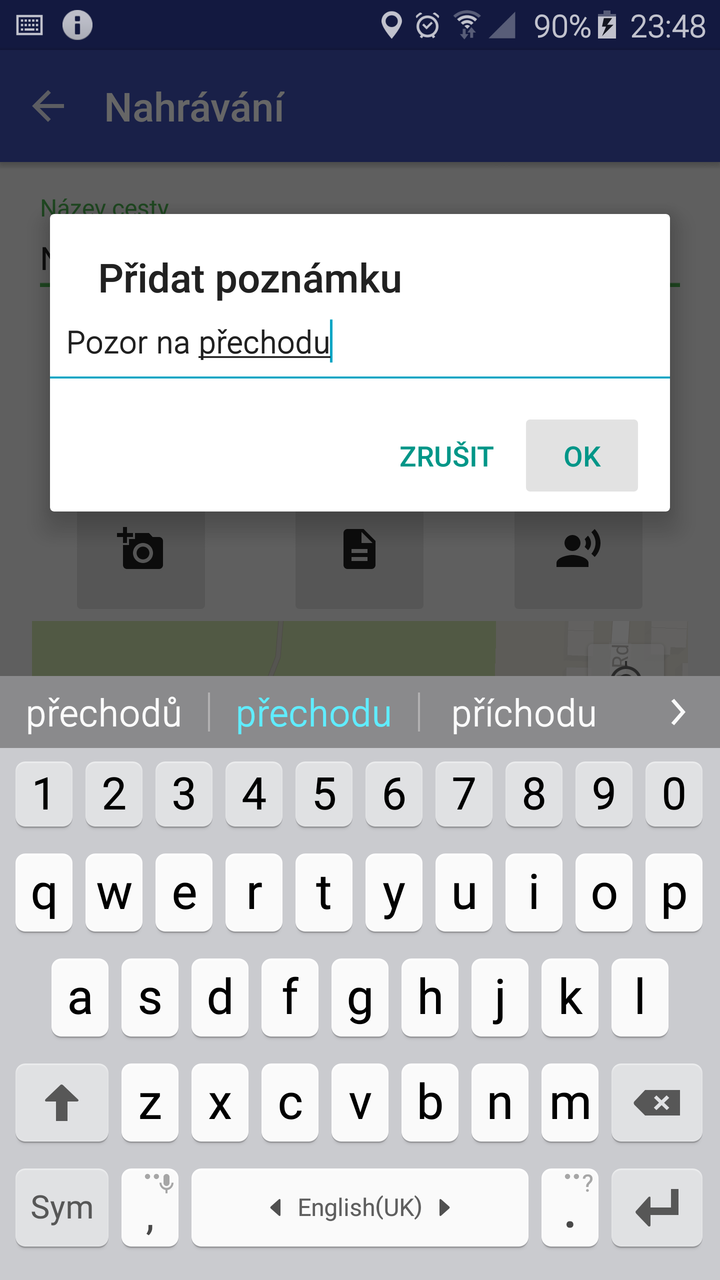
\includegraphics[scale=0.14]{img/screen/pridanipoznamky.png}
        \caption{Přidání poznámky}
        \label{fig:pridanipoznamky}
\end{minipage}
\begin{minipage}{.5\textwidth}
  \centering
                  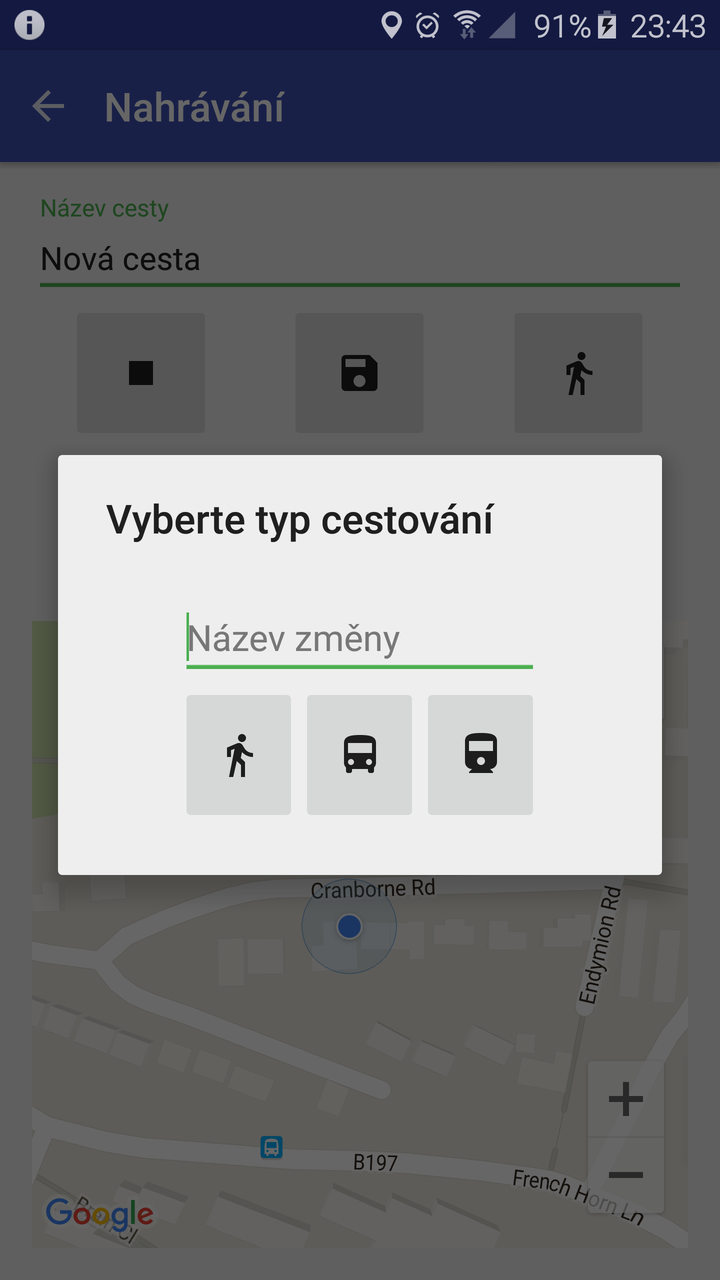
\includegraphics[scale=0.14]{img/screen/zmenaprostredku.png}
          \caption{Změna dopravního prostředku}
          \label{fig:pridanizmenyprostredku}

       \end{minipage}
\end{figure}

\usecase{Přidání změny dopravního prostředku}{pridanizmenyprostredku}
\textbf{Aktéři:} Asistent


\vspace{0.1cm}
\noindent
\textbf{Hlavní scénář:} Zobrazí se okno se nabídkou tlačítek s obrázkem dopravního prostředku.
Uživatel může zároveň přidat ke změně dopravního prostředku přidat popis. Po kliknutí na
tlačítko s dopravním prostředkem se změna dopravního prostředku uloží s asociovanou aktuální polohou
uživatele. Okno změny dopravního prostředku lze vidět na obrázku~\ref{fig:pridanizmenyprostredku}.

\vspace{0.1cm}
\noindent
\textbf{Prekondice:} Uživatel nahrává nebo edituje cestu.

\vspace{0.1cm}
\noindent
\textbf{Spouštěč:} Uživatel klepl na tlačítko s aktuálním dopravním prostředkem.




\usecase{Nahrávání cesty}{nahravanicesty}
\textbf{Aktéři:} Asistent

\vspace{0.1cm}
\noindent
\textbf{Hlavní scénář:} Uživateli se zobrazí nahrávací okno, kde může vidět svou aktuální pozici
a po klepnutí na tlačítko nahrávat začne aplikace sbírat data o poloze a umožní mu přidávat další data
k právě nahrávané pozici. V notifikační liště se objeví notifikace o tom, že aplikace právě nahrává.
Uživatel může v tu chvíli odejít z aplikace, případně navštívit její jiné obrazovky a poté se do nahrávání vrátit,
aniž by ztratil právě nahrávaná data. Stejně tak po opuštění aplikace při nahrávání se do ní může vrátit
klepnutím na zobrazenou notifikaci.

Na mapě vidí uživatel dosud nahranou a uloženou cestu a případné přidané data.
Klepnutím na tlačítko uložit se aktuálně nahraní data a média uloží, případně aktualizují.
Pokud uživatel dokončil nahrávání cesty, klepne na tlačítko uložit a poté tlačítkem stop zastaví nahrávání,
notifikace zmizí a cesta je v seznamu cest připraveno pro spuštění asistence, případně následnou editaci.
Pokud uživatel ukončí nahrávání bez uložení, je na toto upozorněn a při potvrzení ukončení jsou nahraná data
smazána. Obrazovku nahrávání můžeme vidět na obrázku~\ref{fig:nahravanicesty} a zobrazenou notifikaci
na obrázku~\ref{fig:notifikacenahravanicesty}.

\vspace{0.1cm}
\noindent
\textbf{Prekondice:} Uživatel má v telefonu povolené získávání polohy pomocí GPS.

\vspace{0.1cm}
\noindent
\textbf{Spouštěč:} Uživatel klepne na tlačítko nahrávat v seznamu nahraných cest.

\vspace{0.1cm}
\noindent
\textbf{Rozšíření:}
\begin{itemize}
  \item \nameref{pridanifotky}
  \item \nameref{pridaninahravky}
  \item \nameref{pridanipoznamky}
  \item \nameref{pridanizmenyprostredku}
  \item \nameref{odebranifotky}
  \item \nameref{odebraninahravky}
  \item \nameref{odebranipoznamky}
  \item \nameref{odebranizmenyprostredku}
\end{itemize}

\begin{figure}[H]
\begin{minipage}{.5\textwidth}


        \centering
                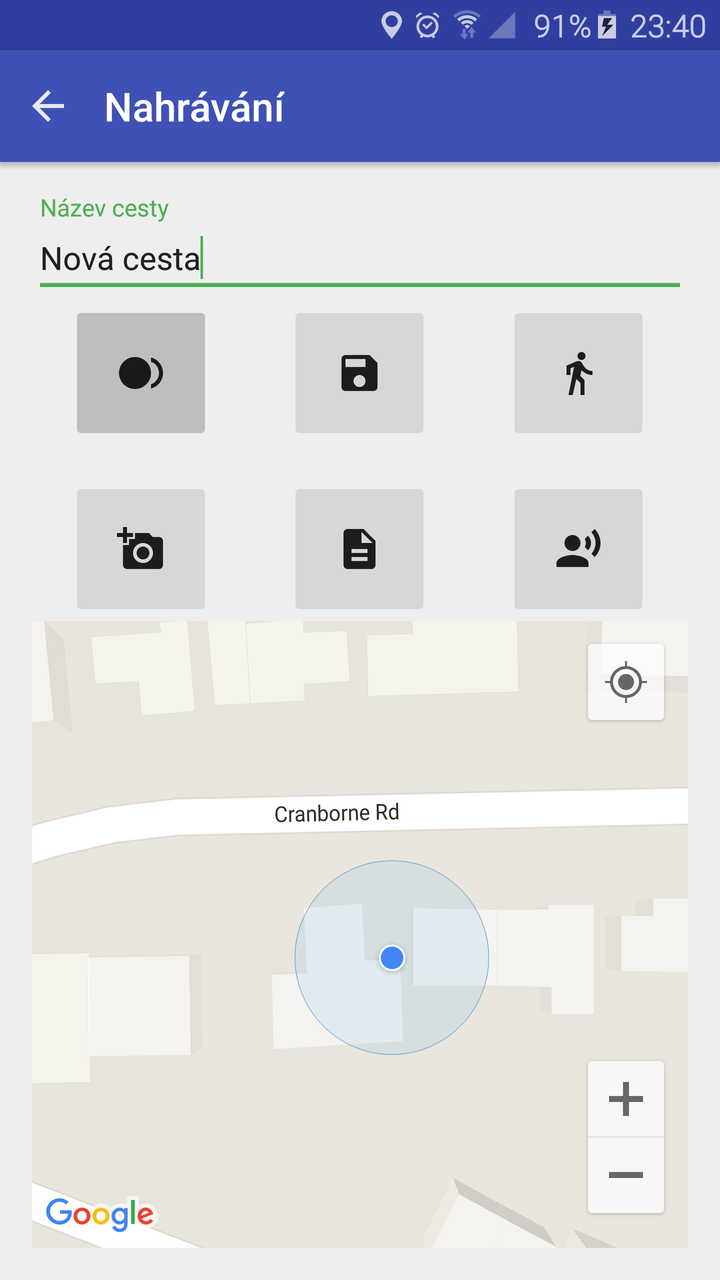
\includegraphics[scale=0.14]{img/screen/nahravani.png}
        \caption{Nahrávání cesty}
        \label{fig:nahravanicesty}
\end{minipage}
\begin{minipage}{.5\textwidth}
  \centering
                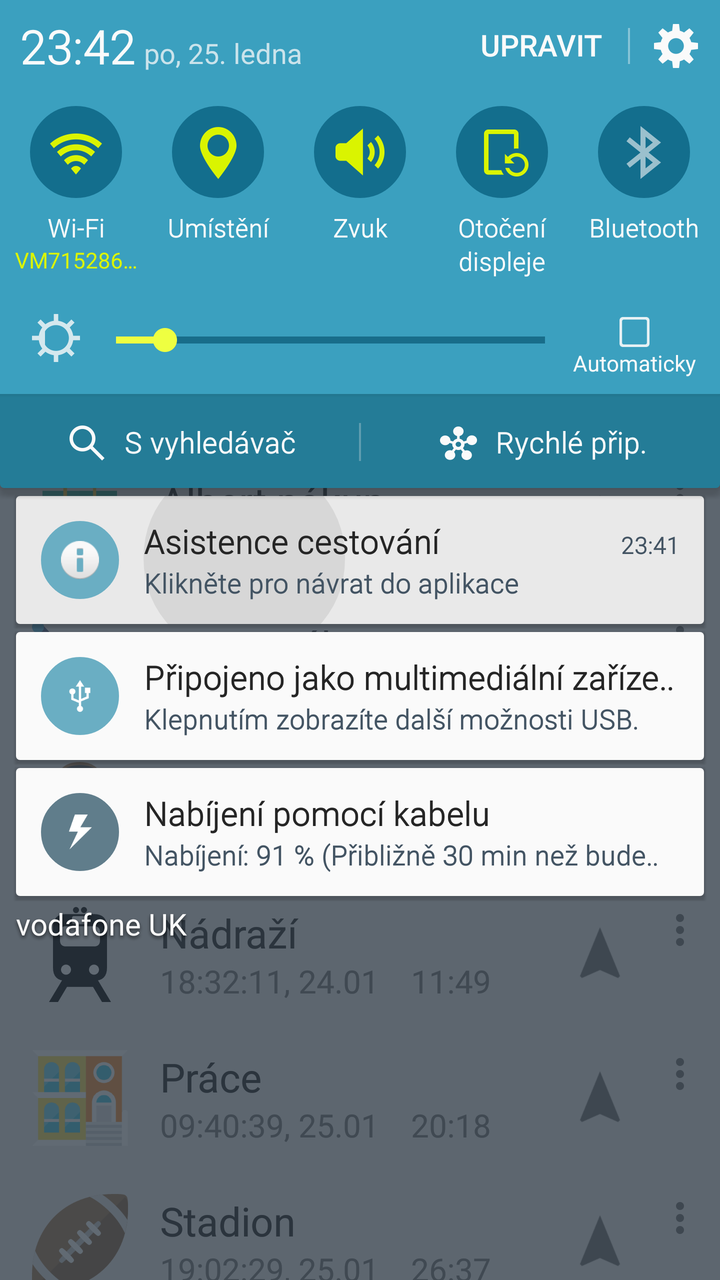
\includegraphics[scale=0.14]{img/screen/notifikace.png}
        \caption{Zobrazená notifikace}
        \label{fig:notifikacenahravanicesty}

       \end{minipage}
\end{figure}


\usecase{Odebrání fotky}{odebranifotky}
\textbf{Aktéři:} Asistent

\vspace{0.1cm}
\noindent
\textbf{Hlavní scénář:} Uživateli se zobrazí okno s dotazem zda chce fotku odebrat. Po klepnutí na
potvrzovací tlačítko je fotka smazána z úložiště a odstraněna její miniatura z aktuální cesty.

\vspace{0.1cm}
\noindent
\textbf{Prekondice:} Uživatel nahrává nebo edituje cestu a má uloženou fotografii.

\vspace{0.1cm}
\noindent
\textbf{Spouštěč:} Uživatel podrží prst na miniatuře fotografie a vybere možnost smazat.



\usecase{Odebrání zvukové nahrávky}{odebraninahravky}
\textbf{Aktéři:} Asistent

\vspace{0.1cm}
\noindent
\textbf{Hlavní scénář:} Uživateli se zobrazí dotaz zda chce nahrávku opravdu smazat, po potvrzení
se uložená nahrávka odstraní a zmizí její ikona.

\vspace{0.1cm}
\noindent
\textbf{Prekondice:} Uživatel nahrává nebo edituje cestu a má uloženou nahrávku.

\vspace{0.1cm}
\noindent
\textbf{Spouštěč:} Uživatel podrží prst na ikoně nahrávky a vybere možnost smazat.



\usecase{Odebrání poznámky}{odebranipoznamky}
\textbf{Aktéři:} Asistent

\vspace{0.1cm}
\noindent
\textbf{Hlavní scénář:} Uživateli se zobrazí okno s dotazem na smazání poznámky. Po potvrzení se
nahrávka smaže a zmizí ikona indikující nahrávku.

\vspace{0.1cm}
\noindent
\textbf{Prekondice:} Uživatel nahrává nebo edituje cestu a má uloženou poznámku.

\vspace{0.1cm}
\noindent
\textbf{Spouštěč:} Uživatel podrží prst na ikoně poznámky a vybere možnost smazat.


\usecase{Odebrání změny dopravního prostředku}{odebranizmenyprostredku}
\textbf{Aktéři:} Asistent

\vspace{0.1cm}
\noindent
\textbf{Hlavní scénář:} Uživateli se zobrazí okno s dotazem na smazání změny dopravního prostředku.
Po potvrzení se nahrávka smaže a zmizí ikona indikující nahrávku. Zobrazené nstavení údajů
lze vidět na obrázku~\ref{fig:nastaveniudaju}.

\vspace{0.1cm}
\noindent
\textbf{Prekondice:} Uživatel nahrává nebo edituje cestu a má uloženou změnu dopravního prostředku.

\vspace{0.1cm}
\noindent
\textbf{Spouštěč:} Uživatel podrží prst na ikoně změny dopravního prostředku a vybere možnost smazat.


\usecase{Nastavení údajů asistenta}{nastaveniudaju}
\textbf{Aktéři:} Asistent

\vspace{0.1cm}
\noindent
\textbf{Hlavní scénář:} Uživateli se zobrazí obrazovka s nastavením údajů, kde může vyplnit své údaje.

\vspace{0.1cm}
\noindent
\textbf{Spouštěč:} Uživatel klepl na tlačítko nastavení.

\vspace{0.1cm}
\noindent
\textbf{Rozšíření:}
\begin{itemize}
  \item \nameref{nastavenicisla}
  \item \nameref{nastaveniemailu}
\end{itemize}

\begin{figure}[H]
\begin{minipage}{.5\textwidth}
\centering
                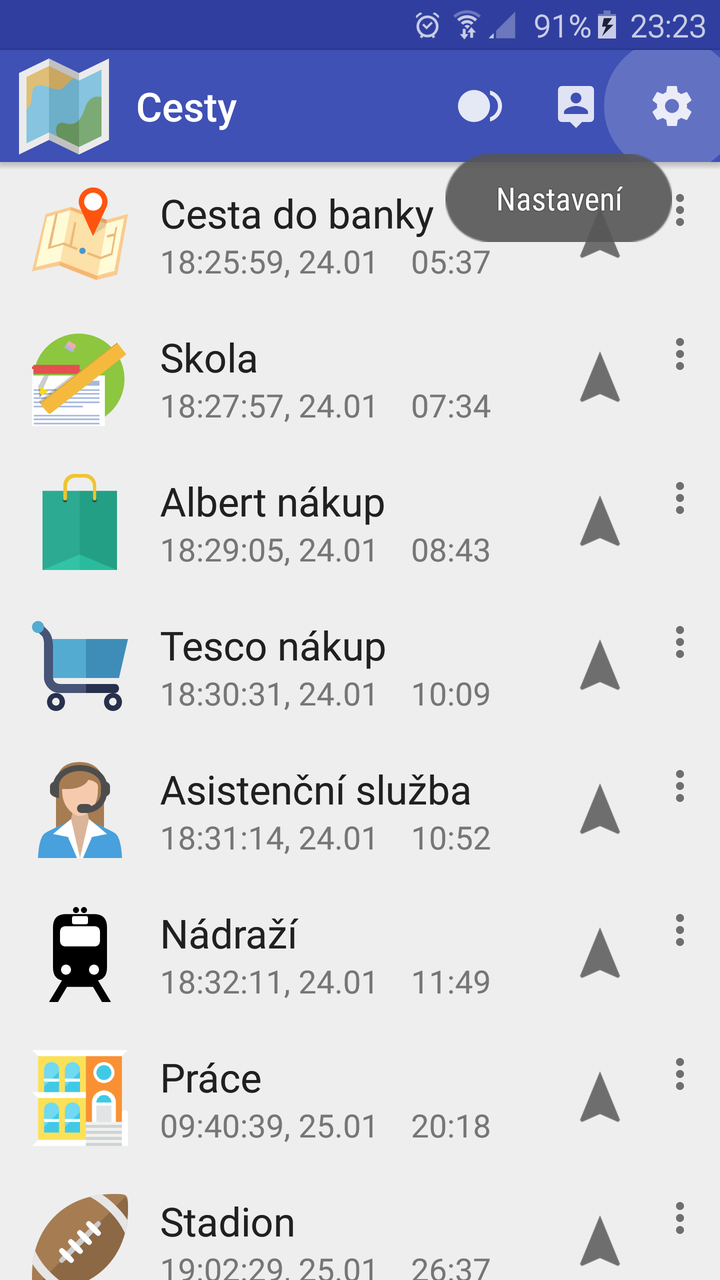
\includegraphics[scale=0.14]{img/screen/nastaveni.png}
        \caption{Spuštění nastavení údajů}
        \label{fig:nastaveniudaju}
\end{minipage}
\begin{minipage}{.5\textwidth}
\centering
                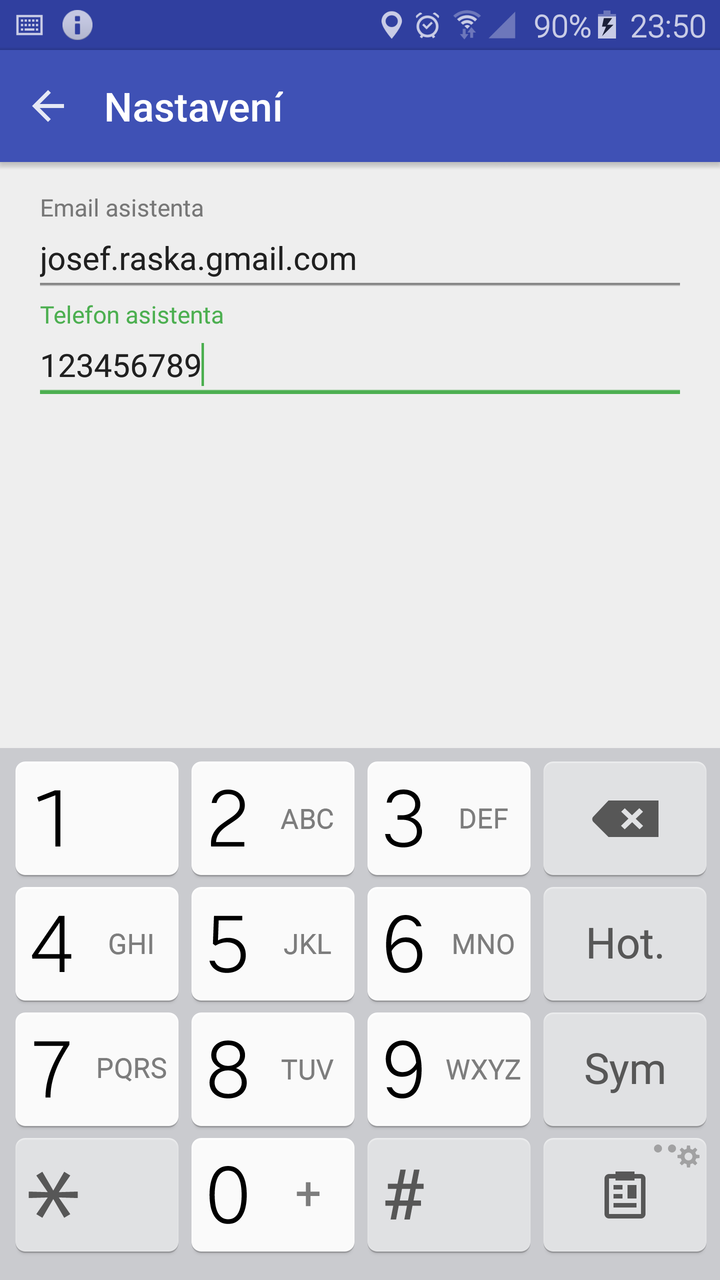
\includegraphics[scale=0.14]{img/screen/nastaveniasistent.png}
        \caption{Nastavení telefonního čísla}
        \label{fig:nastavenicisla}
    \end{minipage}
\end{figure}

\usecase{Nastavení telefonního čísla asistenta}{nastavenicisla}
\textbf{Aktéři:} Asistent

\vspace{0.1cm}
\noindent
\textbf{Hlavní scénář:} Editovatelné pole pro telefonní číslo se zvýrazní a vysune se numerická klávesnice.
Uživatel zadá své telefonní číslo, které se automaticky formátuje do přívětivějšího formátu. Po ukončení
editace je telefonní číslo automaticky uloženo. Pokud telefonní číslo neodpovídá formátu telefonních čísel
v České Republice, uživatel je na toto upozorněn a je vyzván k úpravě vstupu. Zadávání telefonního čísla
vidíme na obrázku~\ref{fig:nastavenicisla}.

\vspace{0.1cm}
\noindent
\textbf{Spouštěč:} Uživatel klepl na editační pole s telefonním číslem asistenta.

\usecase{Nastavení emailu asistenta}{nastaveniemailu}
\textbf{Aktéři:} Asistent

\vspace{0.1cm}
\noindent
\textbf{Hlavní scénář:} Editovatelné pole pro emailovou adresu se zvýrazní a vysune se klávesnice.
Uživatel zadá svou emailovou adresu. Po ukončení editace je emailová adresa automaticky uložena.
Pokud emailová adresa neodpovídá správnému formátu emailové adresy, uživatel je na toto upozorněn
a vyzván k úpravě vstupu.

\vspace{0.1cm}
\noindent
\textbf{Spouštěč:} Uživatel klepl na editovatelné pole emailové adresy.


\usecase{Nastavení zamčení editace}{nastavenizamceni}
\textbf{Aktéři:} Asistent

\vspace{0.1cm}
\noindent
\textbf{Hlavní scénář:} Uživateli se zobrazí editovatelné pole, kde může zadat heslo pro zamčení editace
obsahu aplikace. Pokud toto heslo nezadá, aplikace bude stále v módu editace a uložená data bude možné upravit.
Uživatel zadá heslo, to bude uloženo a bude nyní vyžadováno pro zpřístupnění úprav cest, případně nastavení.

\vspace{0.1cm}
\noindent
\textbf{Spouštěč:} Uživatel klepl na tlačítko nastavení zamčení.

\usecase{Nastavení zálohování}{nastavenizalohovani}
\textbf{Aktéři:} Asistent

\vspace{0.1cm}
\noindent
\textbf{Hlavní scénář:} Uživateli se zobrazí výběr z listu zda chce zálohovat manuálně, jednou za den, týden
nebo za měsíc. Uživatel vybere jednu z možností a podle výběru se naplánují příslušné akce.

\vspace{0.1cm}
\noindent
\textbf{Prekondice:} Uživatel má na zařízení nastaven účet umožňující zálohování.

\vspace{0.1cm}
\noindent
\textbf{Spouštěč:} Uživatel klepl na tlačítko nastavení zálohování.


















\subsection{Use casy uživatele Klient}
Pro klienta jsou určeny více intuitivní a nenáročné operace vyžadující co nejméně aktivních
kroků z klientovi strany. Aplikace by měla na základě polohy a dalších údajů sama rozpoznat,
co má v danou chvíli udělat. Use casy klienta a jejich vztahy lze vidět na obrázku~\ref{fig:UseCasesClient}.

\begin{figure}[H]
        \centering
                \includegraphics[scale=0.2]{img/UseCasesClient.png}
        \caption{Diagram use casů uživatele klient}
        \label{fig:UseCasesClient}
\end{figure}


\usecase{Prohlížení seznamu nahraných cest}{prohlizeniklient}
\textbf{Aktéři:} Klient

\vspace{0.1cm}
\noindent
\textbf{Hlavní scénář:} Na úvodní obrazovce jsou pod sebou vyobrazeny všechny cesty, pro které může
uživateli aplikace poskytnout asistenci. Uživatel si prohlíží cesty, které mají zobrazeny pouze
základní informace a jsou označeny vybraným obrázkem pro snažší orientaci. Uživatel si poklepnutím
na řádek cesty může dostat na její detail případně rychlými akcemi spustí navigaci.

\vspace{0.1cm}
\noindent
\textbf{Spouštěč:} Uživatel klepne na ikonu aplikace v telefonu.

\vspace{0.1cm}
\noindent
\textbf{Rozšíření:}
\begin{itemize}
  \item \nameref{detailklient}
  \item \nameref{asistence}
\end{itemize}

\usecase{Detail nahrané cesty}{detailklient}
\textbf{Aktéři:} Klient

\vspace{0.1cm}
\noindent
\textbf{Hlavní scénář:} Klientovi se zobrazí obrazovka se všemi údaji, které mu mají na cestě pomoci.
Fotky jsou vidět jako miniatury na místě, kde byly pořízeny, podobně nahrávky, změny dopravního prostředku
a poznámky, které jsou reprezentovány svými příslušnými jednoduchými ikonami.

\vspace{0.1cm}
\noindent
\textbf{Prekondice:} Uživatel má nahranou cestu.

\vspace{0.1cm}
\noindent
\textbf{Spouštěč:} Uživatel klepne na řádek cesty v seznamu nahraných cest.

\vspace{0.1cm}
\noindent
\textbf{Rozšíření:}
\begin{itemize}
  \item \nameref{asistence}
\end{itemize}


\usecase{Asistence cestování}{asistence}
\textbf{Aktéři:} Klient

\vspace{0.1cm}
\noindent
\textbf{Hlavní scénář:} Uživateli se zobrazí jednoduchá mapka s vyznačenou cestou, kterou má absolvovat.
Zobrazí se mu všechny dostupné informace jako čas do cíle, doporučený směr, nejbližší nahrané fotky,
nahrávky nebo poznámky. Zkontroluje se podle uložených statistik, zda bude uživateli stačit baterie
k absolvování cesty a pokud ne, bude na to upozorněn.
Aplikace využívá klientovu polohu pro zobrazení relevantních nahraných informací
a snaží se mu napovídat následující směr pomocí zobrazené šipky. Jak se klient pohybuje, aplikace mu
poskytuje nahraný obsah asistentem, který by mu měl pomoci v danou chvíli se lépe zorientovat.
Obrazovku asistence cestování lze vidět na obrázku~\ref{fig:asistence}.

\vspace{0.1cm}
\noindent
\textbf{Prekondice:} Klient má nahranou cestu a spustil asistenci cestování po této cestě.

\vspace{0.1cm}
\noindent
\textbf{Spouštěč:} Klient klepl na obrázek navigovat.

\vspace{0.1cm}
\noindent
\textbf{Rozšíření:}
\begin{itemize}
  \item \nameref{zobrazenifotky}
  \item \nameref{prehraninahravky}
  \item \nameref{zobrazenipoznamky}
  \item \nameref{upozorneniprostredek}
  \item \nameref{analyzabaterie}
  \item \nameref{zobrazenismeru}
  \item \nameref{upozorneninespravnysmer}
\end{itemize}


\begin{figure}[H]
\begin{minipage}{.5\textwidth}
\centering
                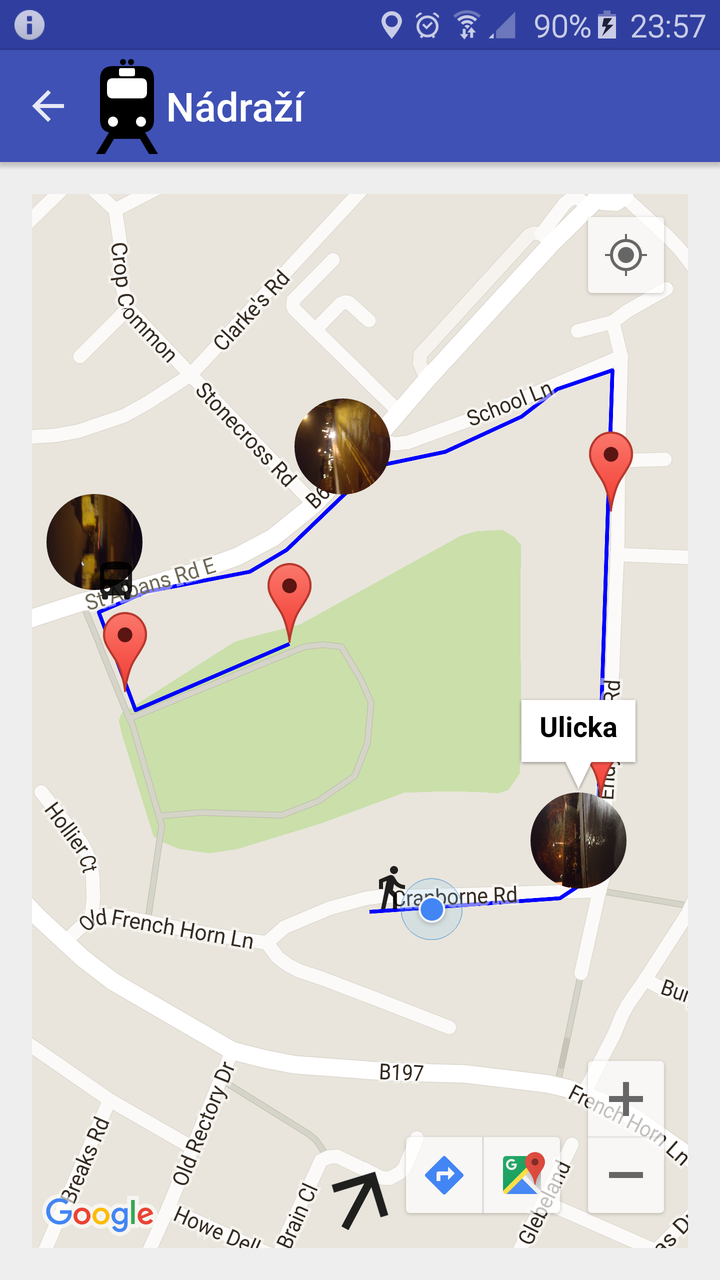
\includegraphics[scale=0.14]{img/screen/asistencecestovani.png}
        \caption{Asistence cestování}
        \label{fig:asistence}
\end{minipage}
\begin{minipage}{.5\textwidth}
\centering
                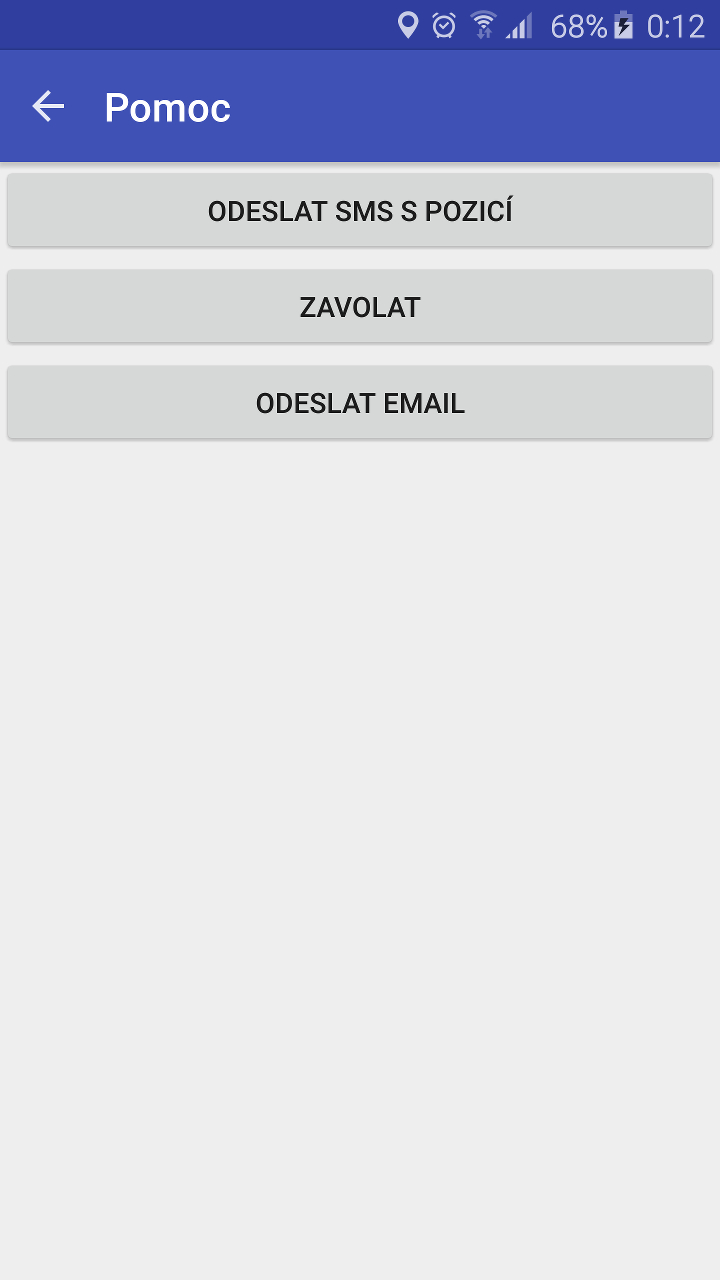
\includegraphics[scale=0.14]{img/screen/volanipomoc.jpg}
        \caption{Obrazovka pomoci}
        \label{fig:pomoc}
    \end{minipage}
\end{figure}



\usecase{Zobrazení fotografie}{zobrazenifotky}
\textbf{Aktéři:} Klient

\vspace{0.1cm}
\noindent
\textbf{Hlavní scénář:} Uživatel se přiblíží k místu pořízení fotografie, aplikace toto rozpozná
a upozorní uživatele na přítomnost fotky, která se zobrazí na dobu, po kterou je uživatel nablízku.
Přes spodní část fotky je zobrazen popisek, který této fotce dříve zadal asistent.

\vspace{0.1cm}
\noindent
\textbf{Prekondice:} Uživatel má k dané cestě uloženou fotku.

\vspace{0.1cm}
\noindent
\textbf{Spouštěč:} Uživatel se přiblíží místu pořízení fotky nebo klepne na miniaturu fotky.


\usecase{Přehrání uložené zvukové nahrávky}{prehraninahravky}
\textbf{Aktéři:} Klient

\vspace{0.1cm}
\noindent
\textbf{Hlavní scénář:} Uživatel se se zapnutou asistencí cestování přiblíží místu,
kde byla dríve za pomoci asistenta pořízena zvuková nahrávka. Uložená nahrávka se načte
a začne se uživateli přehrávat. Zároveň se zobrazí popis nahrávky a tlačítko umožňující
nahrávku přehrát znovu.

\vspace{0.1cm}
\noindent
\textbf{Prekondice:} Uživatel má k dané cestě uloženou zvukovou nahrávku.

\vspace{0.1cm}
\noindent
\textbf{Spouštěč:} Uživatel se přiblíží k místu pořízení nahrávky nebo klepne na ikonu nahrávky.

\usecase{Zobrazení uložené poznámky}{zobrazenipoznamky}
\textbf{Aktéři:} Klient

\vspace{0.1cm}
\noindent
\textbf{Hlavní scénář:} Uživatel je při přiblížení se místu poznámky upozorněn a poznámka se zobrazí.

\vspace{0.1cm}
\noindent
\textbf{Prekondice:} Uživatel má k dané cestě uloženou poznámku.

\vspace{0.1cm}
\noindent
\textbf{Spouštěč:} Uživatel se přiblíží k místu pořízení poznámky nebo klepne na ikonu poznámky.

\usecase{Upozornění na změnu dopravního prostředku}{upozorneniprostredek}
\textbf{Aktéři:} Klient

\vspace{0.1cm}
\noindent
\textbf{Hlavní scénář:} Uživateli je při přiblížení ke změně dopravního prostředku upozorněn,
zobrazí se mu obrázek dopravního prostředku, do kterého má nastoupit nebo naopak vystoupit spolu
s textem, který byl při nahrávání cesty zadán.

\vspace{0.1cm}
\noindent
\textbf{Prekondice:} Uživatel má uloženo upozornění na změnu dopravního prostředku.

\vspace{0.1cm}
\noindent
\textbf{Spouštěč:} Uživatel se přiblíží k místu změny dopravního prostředku.



\usecase{Analýza spotřeby baterie}{analyzabaterie}
\textbf{Aktéři:} Klient

\vspace{0.1cm}
\noindent
\textbf{Hlavní scénář:} Během cestování se ukládají průběžně data o spotřebě beterie a délce trvání
cesty. Data jsou poté spolu s předchozími záznamy statisticky analyzována a je odhadována a upřesňována
očekávaná výdrž baterie během navigace. Na základě těchto analýz může být uživatel poté upozorněn na
nebezpečí vybití baterie v terénu.

\vspace{0.1cm}
\noindent
\textbf{Spouštěč:} Uživatel využívá asistence při cestování.



\usecase{Zobrazení doporučeného směru}{zobrazenismeru}
\textbf{Aktéři:} Klient

\vspace{0.1cm}
\noindent
\textbf{Hlavní scénář:} Na základě pohybu uživatele jsou data vyhodnocována a vypočítán aktuální směr uživatele.
Ten se porovná s očekávaným a uloženým směrem a podle rozdílu se zobrazí směr, kterým by se uživatel měl ideálně
vydat. Informace je zobrazena v dolní části obrazovky v podobě jednoduché šípky.

\vspace{0.1cm}
\noindent
\textbf{Prekondice:} Uživatel se pohybuje po cestě nebo chodníku.

\vspace{0.1cm}
\noindent
\textbf{Spouštěč:} Uživatel využívá asistence při cestování.


\usecase{Upozornění na nesprávný směr}{upozorneninespravnysmer}
\textbf{Aktéři:} Klient

\vspace{0.1cm}
\noindent
\textbf{Hlavní scénář:} Když se uživatel nepohybuje dle očekávané trasy, aplikace může vyhodnotit
tento pohyb jako nesprávný. V takovém případě začne uživatele upozorňovat a pokud směr nezmění nebo
neklepne na tlačítko známý směr, bude s upozorňováním pokračovat a nabízet směr správný.

\vspace{0.1cm}
\noindent
\textbf{Spouštěč:} Uživatel se během asistence cestování určitou dobu pohybuje jiným, než očekávaným směrem.


\usecase{Spuštění asistence cestování po přiložení NFC tagy k telefonu}{prilozeninfc}
\textbf{Aktéři:} Klient

\vspace{0.1cm}
\noindent
\textbf{Hlavní scénář:} Klient přiloží telefon k nálepce, kartě nebo čemukoliv jinému, co bylo použito
jako NFC tag a obsahuje informace o cestě. Tato informace se přečte a spustí se aplikace se zapnutou
asistencí cestování na cestu zapsanou na tagu.

\vspace{0.1cm}
\noindent
\textbf{Prekondice:} Klient má k dispozici NFC tag, na který byla dříve zapsána informace o cestě.

\vspace{0.1cm}
\noindent
\textbf{Spouštěč:} Klient přiloží telefon k NFC tagu.

\vspace{0.1cm}
\noindent
\textbf{Rozšíření:}
\begin{itemize}
  \item \nameref{pridanifotky}
\end{itemize}

\usecase{Vyvolání obrazovky pomoci}{pomoc}
\textbf{Aktéři:} Klient

\vspace{0.1cm}
\noindent
\textbf{Hlavní scénář:} Uživateli se zbrazí obrazovka s volbami rychlých akcí,
které kontaktují jeho asistenta. Obrazovka pomoci je na obrázku~\ref{fig:pomoc}.

\vspace{0.1cm}
\noindent
\textbf{Prekondice:} V zařízení jsou uloženy kontaktní údaje asistenta.

\vspace{0.1cm}
\noindent
\textbf{Spouštěč:} Uživatel klepne na obrázek pomoc v aplikaci.

\vspace{0.1cm}
\noindent
\textbf{Rozšíření:}
\begin{itemize}
  \item \nameref{pomocvolani}
  \item \nameref{pomocsms}
  \item \nameref{pomocemail}
\end{itemize}



\usecase{Volání asistentovi}{pomocvolani}
\textbf{Aktéři:} Klient, Asistent

\vspace{0.1cm}
\noindent
\textbf{Hlavní scénář:} Uživateli se zobrazí obrazovka, kde vidí vytáčení čísla na svého asistenta.
Hovor se poté uskuteční.

\vspace{0.1cm}
\noindent
\textbf{Prekondice:} V aplikaci je uloženo telefonní číslo asistenta.

\vspace{0.1cm}
\noindent
\textbf{Spouštěč:} Uživatel klepne na číslo asistenta.

\usecase{Poslání SMS zprávy s aktuální polohou}{pomocsms}
\textbf{Aktéři:} Klient, Asistent

\vspace{0.1cm}
\noindent
\textbf{Hlavní scénář:} Uživateli se zobrazí potvrzení o odeslání SMS zprávy a její znění.
Asistentovi se zobrazí zpráva, ve které je také odkaz na mapu s GPS polohou klienta v době odesílání zprávy.

\vspace{0.1cm}
\noindent
\textbf{Prekondice:} V aplikaci je uloženo telefonní číslo asistenta.

\vspace{0.1cm}
\noindent
\textbf{Spouštěč:} Uživatel klepne na tlačítko poslat SMS.


\usecase{Poslání emailu s aktuální polohou}{pomocemail}
\textbf{Aktéři:} Klient, Asistent

\vspace{0.1cm}
\noindent
\textbf{Hlavní scénář:} Kientovi se otevře emailová aplikace s nachystanou zprávou a adresou asistenta
a klient klepne odeslat. Asistentovi přijde email s žádostí o pomoc a odkazem na mapu s GPS polohou
klienta v době odeslání emailu.

\vspace{0.1cm}
\noindent
\textbf{Prekondice:} V aplikaci je uložena emailová adresa asistenta.

\vspace{0.1cm}
\noindent
\textbf{Spouštěč:} Uživatel klepne na tlačítko odeslat email.









\subsection{Použité nástroje}
\subsubsection{draw.io (http://www.draw.io)}
Online nástroj pro tvorbu grafů, všech různých typů diagramů, myšlenkových map a dalších.
Celý editor běží pouze v prohlížeči a synchronizuje vytvářené grafy s připojeným úložištěm
Google Drive nebo Dropbox. Grafy jsou tak přístupné  a editovatelné odkudkoliv a aplikace
je opravdu pokročilá a při práci není vůbec poznat, že vše probíhá pouze v prohlížeči.
Umožňuje sdílení i export zhotovených diagramů do mnoha formátů a je tedy velice snadné
sdílet a používat vytvořenou práci.
Nástroj byl použit pro vytváření use case diagramů a třídních diagramů v této práci.
\begin{figure}[H]
        \centering
                
\includegraphics[scale=0.2]{img/drawiologo.png}
        \caption{Logo nástroje draw.io}
        \label{fig:iologo}
        \centering Zdroj: \url{http://www.draw.io}
\end{figure}



\section{Implementace}

\subsection{Použité nástroje pro vývoj}
Android je v současné době nejpoužívanější mobilní operační systém a programuje pro něj obrovské
množství vývojářů, kteří pro stále vyšší nároky na aplikace potřebují pracovat efektivně a Android samotný
a spoustu dalších společností pro ně poskytuje celou řadu nástrojů, které jim mají usnadnit práci a zefektivnit vývoj.

\subsubsection{Vývojové prostředí}
Přesto, že první verze Andorid vyšla již před 10 lety, získal Android své vlastní vývojové prostředí, Android Studio,
až v roce 2013 a na verzi 1.0 si vývojáři počkali až do konce roku 2014. Dříve býl vývoj řešen pluginy ve známých
vývojovoých prostředích jako Eclipse, NetBeans a pozdějí IntelliJ IDEA od JetBrains. Právě poslední jmenované
se časem stalo jedničkou a díky tomu, že existuje open source verze, posloužila IntelliJ jako základ pro Android Studio
a dodnes se změny pro IntelliJ dostávají postupně do Android Studia a naopak, takže se vzájemně stále obohacují.

S příchodem vlastního vývojového prostředí se vývoj značně zjednodušil a tým Andorid Studia neustále vylepšuje integraci s SDK,
nástroji pro sestavení, neboli build projektu a pluginy, kterých je celá řada a ten hlavní je Android Gradle Plugin
nad open source build systémem Gradle, umožňujícímu definici buildu v Groovy skriptech s možností využití Javy,
 pomocí něhož se celý projekt sestavuje a vytváří se aplikace se všemi dílčími kroky, které jsou pro to potřeba.
Pomocí Gradle pluginu se do procesu sestavení tyto kroky vloží, umožní se jejich konfigurace pomocí Gradle skriptů
a Android Studio slouží pouze jako obálka nad běžícím Gradle buildem, kdy vývojové prostředí řeší pouze nápovědy vývojáři,
napovídání, analýzu kódu a celkově vývojářovo pohodlí, neřeší však samotný build, který přenechává Gradlu a spuštění buildu
 z příkazové řádky je naprosto ekvivalentní buildu ve vývojovém prostředí, což znamená velkou výhodu při sestavování aplikace
 v cizích prostředích, například build serveru.
 Gradle také poskytuje velice užitečný mechanismus jménem Gradle Wrapper, což je spustitelný Java jar archiv,
 který je spolu s několika skripty uložen spolu s projektem a při spouštění buildu přes tyto skripty stáhne v rámci
 buildu nakonfigurovanou distribuci Gradlu na spouštějící stanici. Při distribuci kódu tedy stačí pouze spustit
 skript a vývojář se nemusí starta o jakoukoliv komplikovanou instalaci build systému.

 \subsubsection{Verzování kódu}
 Jako systém verzování byl použit Git, který je jeden z nejrozšířenějších verzovacích systémů a služba GitHub\url{https://github.com}.
 podporuje zdarma hostování open source repozitářů s nabídkou mnoha služeb okolo, mimo jiné snadnou intergaci se službou
 Travis CI, která byla použita pro průběžnou integraci projektu. Díky službě GitHub je zajištěno zálohování kódu
 během vývoje a díky Gitu je vyřešeno verzování se všemi výhodami, které to s sebou přináší, jaok možnst vráti se
 ke konkrétní verzi projektu, porovnávat a sledovat změny, případně vyvíjet několik funkcionalit nezávisle na sobě.
 Dále bylo pomocí těchto nástorjů řešeno uzavírání verzí publikováno na Google Play, kdy byl pro každou verzi vytvořen
 release, takže v případě, že se objeví problém u uživatele, jsme vždy schopní snadno dostat kód do stavu
 ve kterém je u uživatele a snáze tak najít a vyřešit problém. Stránku projektu na GitHubu lze nalézt na
 \url{https://github.com/jraska/Diploma-Thesis}.

 \subsubsection{Průběžná intergace}
 Díky hostování projektu na GitHubu bylo možné snadné využití službu Travis CI(\url{https://travis-ci.org}),
 která se zaregistruje pro repozitář
 a při každé změně spustí build celého projektu v uzavřeném prostředí, díky čemuž dokážeme okamžitě
 odhalit jakékoliv problémy, které se na naší stanici nemusí projevit, nicméně mimo naše prostředí ano.
 Služba stáhne veškerý kód z repozitáře, nakonfiguruje uzavřený virtuální kontejner, nainstaluje Javu, Android SDK,
 případně další komponenty a spustí build projektu, v rámci něhož se spouští i unit testy. Služba se konfiguruje pomocí
 soubor \texttt{travis.yml} v kořenovém adresáři repozitáře, v němž je specifikováno, že se projekt má sestavit jako Android projekt,
 jaký software se do prostředí má před každým během nainstalovat a co se má stát v případě chyby. Travis CI po stažení
 repozitáře tento soubor vyhledá a na základě jeho obsahu provede požadované akce.
 Službu a historii buildů pro aplikaci Asistence cestování si můžeme prohléednou na \url{https://travis-ci.org/jraska/Diploma-Thesis}.

 \subsubsection{Statická analýza kódu}

\noindent
 \textbf{Lint}


 Pro analýzu kódu a odhalování potencionálních chyb, problémů a nepoužívaných souborů je používán Lint,
  což je nástroj, který v projektu kontroluje dodržení sady poskytnutých pravidel a který
  je již součástí build procesu Androidu. Během buildu se vytváří Lint Report
  se všemi varováními a chybami, které byly v projektu nalezeny. Nástroj je konfigurovatelný pomocí
  Gradle skirptů projektu, případně pomocí souboru \texttt{lint.xml}, pomocí něhož lze některé chyby
  vynechat, případně změnit jejich prioritu například z chyby na varování.
  Lint dokáže odhalit spoustu chyb jako třeba zapomenutí potvrzení při editaci nastavení uživatele,
  nezavření databázového kurzoru, přítomnost nepoužitých obrázků v projektu a podobně.
  Jeho další velkou výhodou je rozšiřitelnost, kde si každý může napsat vlastní Lint pravidla pro to, na co chce být upozorněn
  a v případě knihoven začne Android Studio jejich pravidla automaticky používat a zvýrazňovat problémy uživateli
  přímo v editoru.
  Příkladem může být knihovna pro logování Timber, o které je řeč v sekci \ref{todo} a která pomocí Lint pravidel
  kontroluje, zda je použita správně a dokáže tak předejít chybám za běhu.

\noindent
\textbf{Codacy}


Dalším použitám nástrojem je služba Codacy(\url{https://www.codacy.com/}), což je ve své podstatě
automatizována analýza kódu vyhledávající potenciální chyby a problémy, která se spustí po každé změně v kódu
díky opět snadné integraci s GitHubem. Služba odhaluje problémy jako nepoužívaný kód, příliš složité
třídy nebo metody, známé programátorské chyby či bezpečnostní rizika. Po analýze projekt oznámkuje podle
množství nalezených problémů v poměru k množství analyzovaného kódu. Aktuální analýzu projektu si můžeme ptohlédnout
na \url{https://www.codacy.com/app/josef-raska/Diploma-Thesis/dashboard}.

\subsection{Použité knihovny}
Jak již bylo zmíněno, Andorid používá velé množství vývojářů a pr jejich potřebu vzniklo velké množství
z drivé většiny open source knihoven, které se snaží vyřešit a zjednodušit společný problém mnoha vývojářů
a zesnadnit programování pro Android. Knihovny jsou díky tomu, že si může napsat knihovnu prakticky kdokoliv
různých kvalit a je proto nutné si každou napřed prohlédnout před jejím použitím, nicméně díky jejich
otevřenému kódu a hodnocením dalších uživatelů lze již nyní poměrně snadno najít spolehlivou knihovnu na téměř každý
typický problém, který při vývoji aplikací nastává a pročtěním jejího kódu se ujisti, případně inspirovat,
jak dělat danou věc správně.

U některých knihoven je také zdůvodněno, proč jsou používány,
neboť mnohé řeší velice časté problémy vývoje, příčiny problematického kódu a je na nich založena
architektura aplikace.

\subsubsection{Android Support}
Jedná se o základní knihovnu poskytovanou jako součást SDK, která řeší problémy komptibility aplikace
mezi různými verzemi a sjednocuje jejich vzhled. Poskytuje také množství rozšiřujících komponent uživatelského rozhraní,
pomocné třídy například pro notifikace, média a spoustu dalších. V současné době by měla být součástí každě
aplikace a při vytáření nového projektu je k projektu již automaticky přidána.

Dokumentaci knihovny můžeme najít na \url{http://developer.android.com/tools/support-library/index.html}.

\subsubsection{Dagger 2 a vkládání závislostí}
Poměrně nová knihovna spravovaná Googlem a uvolněná poprvé v srpnu 2015, která pro nás řeší tzv. vkládání
závislostí(anglicky Dependecy Injection) do objektů,
které tyto závislosti chtějí používat. Knihovna je použita za účelem zkvalitnění kódu a zlepšení testovatelnosti, jelikož
je v celém projetku následována filozofie, že třídy by měly objekty buď vytvářet a nebo používat. To v podstatě to znamená,
že se snažíme omezit situace, kdy si třída v rámci své metody vytváří vlastní objekty, které potřebuje k vykonání
dané operace a zejména se se snaží úplně elimonovat situace, kdy si třída své závislosti sama začne vybírat z nějakého
kontejneru, statických proměnných a podobně. Jako špatný přístup je v tomto případě brán i často používán návrhový vzor
Jedináček, jelikož se jedná v podstatě o sdílený globální stav. Všechny objekty by měly své závislosti obdržet v konstruktoru
a neměly by se vyskytovat žádné metody tipu inicializuj objekt, nastav proměnnou, bez které objekt nemůže fungovat a podobně.

Cílem tohoto přístupu je zaručit jakémukoliv klientovi třídy, tedy programátorovi používajícímu její rozhraní,
záruku, že pokud získá referenci na tento objekt, bude vždy ve stavu připraveném pro použití a nemůže se mu stát,
že při volání některé z metod obdrží chybu, že zapomněl něco nastavit. Myšlenkou je, že programátor používající
tuto třídu musí pro její použití vidět pouze konstruktor a následně její rozhraní a nemusí pátrat, zda musí po
vytvoření objektu něco nastavovat. Kromě toho tento přístup výrazně zjednodušuje testovatelnost třídy, jelikož v rámci
Android testů běží všechny testy v jednom virtuálním stroji, mají tedy sdílenou paměť, což znamená, že statický
stav zůstává sdílen mezi testy, rozbíjí filozofii izolovanosti testů a může vyústit v situaci, kde jeden test selže,
jelikož nějaký jiný test před ním nastavil něco do globálního stavu.

Často je však tuto filozofii poměrně složité následovat, jelikož aby mohl programátor vytvořit objekt, který
v dané situaci potřebuje, musí mít přístup ke všem jeho závislostem, což může být obtížné zajistit
a vyvstává diskuze, kde odkazy na tyto objekty držet, jak je zpřístupnit všem potenciálním klientům třídy
a jak toto udělat přehledně bez toho, aniž by bylo vše vytvářeno na jednom místě. Toto může vyústit v techniky
jako je lokátor služeb, již zmíněný Jedináček a podobné, kdy si třída sama ve své implementaci potřebnou
závislost vytáhne, čemuž bychom chtěli předejít.
Android nám tento problém také značně stěžuje tím, že hlavní komponenty aplikace jako aktivity, služby a objekt
aplikace samotné jsou provázány co nejvolněji a nelze jednoduše předat jeden objekt z aktivity do aktivity,
dokud se nejedná o primitivní typ, případně jej lze serializovat.

Tento problém pro nás řeší knihovny pro vkládání závislostí, které se nám snaží umožnit to, že si o potřebné
závisloti prostě řekneme a knihovna nám je poskytne. My však musíme knihovně říct, jak tyto závislosti může
získat a kde je má uložit. Dagger 2 používá objekt nazvaný \texttt{Component}, což je kontejner závislostí
který dokáže vytvářet námi požadovené objekty i s jejich závislostmi. Kontejner se skáládá z modulů, které
za podmínky určitých vstupů posktytnou kontejneru nové výstupy. V kódu se tyto třídy definují pomocí anotací
a kód pro vytvoření kontejneru závislotí, nebo také objektového grafu, je vygenerován během kompilace
a díky tomu se za běhu vytvoří velmi rychle, což je jedne z hlavních důvodů, proč je Dagger 2 používá,
protože za běhu vůbec napoužívá reflexi, která je u knihoven tohoto typu častá a která způsobuje v Android
aplikacích značné výkonnostní problémy. Knihovny pro vkládání závislostí existovaly již mnohem dříve,
jako například Spring nebo Guice, při použití na platformě Android byly však díky reflexe pomalé a mohlo snadno
dojít k chybě za běhu. Oproti tomu Dagger 2 vytváří objektový graf během kompilace, zkontroluje zda je acyklický,
všechny požadované závislosti je možné získat a v případě aplikace nám neumožní aplikaci úspěšně zkompilovat,
díky čemuž minimalizuje možné pády aplikace v případě nesprávného použití knihovny.

Dokumentaci a popis knihovny můžeme nalézt na \url{http://google.github.io/dagger/}.

\subsubsection{RxAndroid}
Jedná se o Android rozšíření známé knihovny RxJava, která implementuje reaktivní rozšíření
mnohých programovacích jazyků sdružené pod projekt ReactiveX(\url{http://reactivex.io/}).
Knihovna k Java implementaci pouze přidává vlastnosti specifické pro platformu Android a to konkrétně
řešení spouštění metod v hlavním vlákně uživatelského rozhraní. Knihovna je založena na návrhovém
vzoru Pozorovatel(Observer) a její záměr je implementovat reakce na události bez vědomí, kdy přesně
událost nastane, ale s vědomím, že v tuto chvíly bude registrovaný pozorovatel na tuto událost
upozorněn a zareaguje na ni. Knihovna nabízí spoustu metod, jak na události reagovat, shlukovat je do
skupin, mapovat objekty výsledku na jiné, řeší příliš mnoho požadavků v jednom čase a spostu dalších vlastností.
Jedná se o poměrně mocný nástroj, který nicméně vyžaduje nemálo času na nastudování, pochopení a v případě
Android platformy platí, že s velkou sílou přichází velká zodpovědnost, jelikož při registrace pozorovatele
se často v rámci registrace drží reference na aktivitu, což může v případě například rotace způsobit únik paměti,
případně i pád aplikace v důsledku pokusu o aktualizaci uivatelského rozhraní, které v té době už nemusí být dostupné.

RxAndroid navíc řeší další, pro Andorid velmi významný problém a tím je výběr vlákna, ve kterém se
operace spouští. Jako hlavní vlákno totiž slouží vlákno uživatelského rozhraní, které by
nemělo provádět žádné, byť je trochu náročné operace, neboť by se vše mělo stihnot během 16ms.\cite{perf}
V aplikacích i knihovnách toto vede k obrovskému množství asynchronních zpětných volání, které mají různá jména,
každá knihovna si je řeší po svém, není nad nimi kontrola a výsledkem je nepřehledný asynchronní kód,
ve kterém se lze jen složitě orientovat. Díky RxAndroid a jejich implementaci plánovačů, lze rozhodnutí,
na jakých vláknech bude operace spuštěna a na kterém vlákně bude doručen výsledek nechat na klientovi třídy
a tím pádem například řetězit synchronní volání, pokud jsme již v asynchronním vlákně a zejména zajistit,
že výsledek obržíme ve vlákně uživatelského rozhraní. Typická ukázka využití této vlastnosi
lze vidět na ukázce kódu \ref{rxmainthreaddeliver}, kde se získá seznam cest, operace pro jeho získání,
které jsou časově náročné se spustí v jiném vlákně a výsledek bude doručen na hlavní vlákno,
kde spustí poskytnutou metodu.


\begin{lstlisting}[label=rxmainthreaddeliver,caption=Reakce na událost v UI vlákně pomocí RxAndorid]
    ...
    routesRepository.selectAll()
        .subscribeOn(Schedulers.io())
        .observeOn(AndroidSchedulers.mainThread())
        .subscribe(this::setRoutes);
  }

  void setRoutes(List<RouteData> routes) {...}
\end{lstlisting}

Výhody reaktivního porgramování můžeme ocenit i při testování, které je typicky s asynchronním
rozhraním testované třídy problematické, nicméně díky RxAndroid volání \texttt{toBlocking()} vynutíme
synchronní spuštění požadované operace, což nám výrazně zjednoduší testování.

Knihovnu můžeme nalézt na \url{https://github.com/ReactiveX/RxAndroid}.

\subsection{Architektura}
TODO: IoC, DI, RxJava


TODO: Lombok, RetroLambda, Support Design, Google Play Services, butterkife, Timber, UniversalImageLoader, Okio

\subsection{Ukládaní dat}
Vzor repository, SQLite , DBFlow

\subsection{Zálohování dat}
Jelikož asistent může strávit poměrně dost času sběrem dat a jejich přípravou pro klienta, je žádoucí chránit data před ztrátou,
poškozením nebo pouze nechtěným smazáním či smazáním odinstalací aplikace. Aplikace tudíž obsahuje mechanismus pro zálohu všech
dat a to nahraných cests poznámkami, upozorněními na změnu cesty, fotkami a nahrávkami.

Pro fungující zálohování je nutné přiřadit uživateli identitu a tu rozpoznávat a ověřovat pro přiřazení případná zálohy,
mít k dizpozici webové úložiště, komunikovat s ním a porovnávat informace z něj získané s aktuálními daty,
což je poměrně komplexní úkol a vlastní implementace by
vyžadovala vlastní server, hosting a zejména registraci uživatel, což by v případě mentálně postižených klientů
přineslo další složitost do aplikace a nutilo by klienta pamatovat si další uživatelské jméno a heslo.

Tento problém byl vyřešel využitím OAuth2\footnote{Více o OAuth2 se můžeme dozvědět v \cite{oauth2}.}
autorizace přes připojený Google účet na zařízení a API Google Drive nebo česky Disk,
 které je součástí Google Play Services a na zařízení uživatele, který si naši aplikací stáhnul z obchodu Play,
 jsou tato API k dispozici.
V Google vývojářské konzoli je napřed nutné aktivovat využití Google Drive API pomocí jména balíčku aplikace a SHA-1 hashe
certifikátu, kterým je podepsáno APK aplikace. Na stejném místě lze také nastavit popis, který se pro aplikaci
uživateli zobrazí, když si prohlíží, které aplikace má ke svému Disku připojeny.
Díky API Google Drive je odpovědnost synchronizace dat přesunuta na služby Googlu a pomocí
OAuth2 se využívá existující účet, čímž se odstraňuje nutnost uživatele zakládat a pamatovat
 další identitu a nám zcela eliminuje nutnost starat se o synchronizaci mezi zařízeními a správu jakýchkoliv účtů.
 Uživatel musí při prvním vytvoření zálohy potvrdit, že souhlasí, aby naše aplikace používala jeho Disk.
 API s tímto počítá a při pokusu o vytváření souborů při nutnosti autorizace sám nabídne ke zobrazení
 dialog pro uživatele a následně vrátí výsledek, zda uživatel službu povolil.

 Data záloh jsou ukládána do tzv. appfolderu\cite{driveappfolder}, což je privátní úložiště aplikace
 a uživatel poté v nastavení svého Disku vidí,
  která aplikace tuto službu využívá a kolik dat zabírá, nevidí však konkrétní data.
  Uživatelův pohled po připojení aplikace a zálohování dat můžeme vidět na obrázku~\ref{fig:connecteddrive}.

\begin{figure}[H]
        \centering
                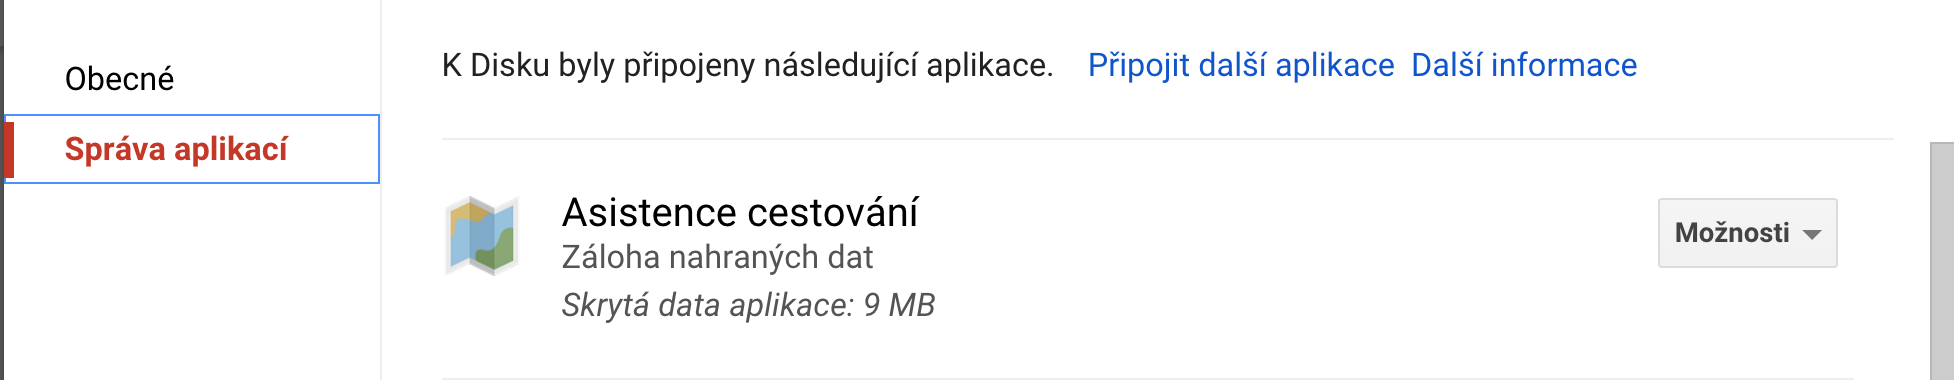
\includegraphics[scale=0.3]{img/connectedDrive.png}
        \caption{Uložená data aplikace na Google Drive}
        \label{fig:connecteddrive}
        \centering Zdroj: \url{https://drive.google.com/drive/my-drive}
\end{figure}

\subsubsection{Záloha}
Pro vytvoření zálohy bylo za účelem minimalizce závislosti na Google Drive API zvoleno vytvoření jediného
dočasného ZIP souboru s databází a soubroy, který se následně uloží na Disk uživatele. Dočasný soubor se po
vytvoření zálohy smaže a stejně tak předchozí zálohy na disku, pro omezení využívání příliš mnoha místa duplicitami,
jelikož díky fotkám může být zálohový soubor poměrně velký. Diagram vytváření zálohy můžeme vidět na obrázku~\ref{fig:backup}.

\begin{figure}[H]
        \centering
                \includegraphics[scale=0.25]{img/backup.png}
        \caption{Diagram vytváření zálohy}
        \label{fig:backup}
\end{figure}

\subsubsection{Obnovení ze zálohy}
Pokud uživatel požádá o obnovení ze zálohy, vyhledá se pomocí Drive API poslední ZIP soubor zálohy,
rozbalí se do dočasného úložiště, soubory se přesunou do příslušných složek, uzavře se existující
databázové připojení aplikace, nahradí se databázový soubor souborem ze zálohy a přípojení se znovu otevře.
Uživatel může následně začít využívat obnovená data.

\subsection{NFC (\textit{Near Field Communication})}
NFC je bezdrátová technolgoie umožňující komunikaci dvou zařízení na velmi krátké vzdálenosti do 4 cm
rychlostí do 424 kb/s.\cite{nfcforum}  Výměna dat může být aktivována pouhým přiblížením dvou zařízení k sobě
a technologie podporuej zabezpečený přenos dat. Technologii spravuje organizace NFC Forum jejíž logo lze vidět
na obrázku \ref{fig:nfcforumlogo} a její specifikaci lze nalézt v \cite{nfciso}.
NFC dále implementuje specifikaci ISO/IEC 14443 A a B\cite{nfcforum}, což je standard používaný
současnými platebními kartami a jinými čipy, jehož definici můžeme najít v \cite{rfidiso} a díky této
implementaci je plně kompatibilní se současnými platebními termínály a systémy, což nabízí možnost využití zařízení
podporujících NFC jako platebních čipů jelikoz oproti klasickým čipům může NFC zařízení uchovávat více informací
a umožňuje například sloučení více platebních karet a bezpečnostních čipů dohromady do jednoho zařízení,
v našem případě mobilního telefonu.

Během posledních pár let se NFC stalo součástí výbavy mnoha chytrých telefonů a velká většina modelů
už nyní tuto funkčnost podporuje a Android nabící ve svém API podporu pro NFC už od verze 2.3
vydané v roce 2010 a vývojář je tedy odstíněn od všech nízkoúrovňových komunikačních protokolů.
V naší aplikaci využijeme tzv. NFC tagů, což je malý vestavěný čip schopný pomocí NFC uchovat malé množství dat a
následně touto technologií tyto data přečíst. Tagy se dají v současnosti koupit na internetu za desítky
korun a mohodu být různých tvarů a barev.

V aplikaci Asistenci Cestování bylo implementováno uložení URL s informací o nahrané cestě. Funkce
pracující s s NFC jsou v aplikaci označeny jednotnou ikonou na obrázku \ref{fig:nfcicon},
která je nejčastěji používána Android aplikacemi.
 Pokud uživatel klepne na ikonu NFC při prohlížení detailu cesty, zobrazí se mu obrazovka s instrukcemi a po přiložení
zapisoatelného NFC tagu je toto URL uložno do tagu spolu s informací, že právě naše aplikace umí toto URL
rozpoznat. V Android Manifestu je následně definována aktivita s intent filtrem na akci \textit{NDEF\_DISCOVERED},
což systému říká, že při objevení NFC tagu má zařadit naši aplikaci na seznam aplikací, které dokážou
rozpoznat NFC tagy a spolu s námi zapsanou informací do tagu je to právě naše aplikace, která při přiložení
tagu zprávu obdrží, dekóduje URL a podle jeho obsahu spustí navigaci nalezené cesty.

Výsledkem je, že uživateli se při přiložení konkrétního tagu zobrazí připravená navigace pro danou
cestu bez jakékoliv další akce, což značně zjednodušuje používání aplikace, jelikož jinak by pro spuštění navigace
uživatel musel aplikaci spustit, nalézt požadovanou cestu a klepnout na ikonku navigace. Nápadem
 využití je přípevnění několika NFC tagů rozlišených barvami vedle dveří bytu klienta a při odchodu na
 cestu uživatel spustí asistenci k cestě přiložením telefonu k požadované barvě.

\begin{figure}[H]
\begin{minipage}{.5\textwidth}
\centering
                
\includegraphics[scale=0.4]{img/nfc-forum-logo.png}
        \caption{Logo organizace NFC Forum}
        \label{fig:nfcforumlogo}
        \centering Zdroj: \url{http://nfc-forum.org/}
\end{minipage}
\begin{minipage}{.5\textwidth}
\centering
                
\includegraphics[scale=0.07]{img/nfc-icon.png}
        \caption{Ikona NFC}
        \centering Zdroj: \url{https://materialdesignicons.com/}
        \label{fig:nfcicon}
    \end{minipage}
\end{figure}


\section{Závěr}


\begin{thebibliography}{99}



\bibitem{perf}{SILLARS, DOUG}
\textit{High Performance Android Apps}. {O'Reilly Media, Inc., 2015}
\newline(Dostupné na \url{https://www.safaribooksonline.com/library/view/high-performance-android/9781491913994/)}

\bibitem{oauth2}{D. HARDT, ED.}
\textit{The OAuth 2.0 Authorization Framework}. {Microsoft, 2012
\newline(Dostupné na \url{https://tools.ietf.org/html/rfc6749})}

\bibitem{driveappfolder}{GOOGLE}.
\textit{Drive API for Android}. {Prosinec 2015,
\newline(Dostupné na \url{https://developers.google.com/drive/android/appfolder})}

\bibitem{nfcforum}{NFC FORUM}.
\textit{About the Technology}. {2016,
\newline(Dostupné na \url{http://nfc-forum.org/what-is-nfc/about-the-technology/})}

\bibitem{nfciso}{ISO/IEC}.
\textit{ISO/IEC 18092}. {2013,
\newline(Dostupné na \url{https://www.iso.org/obp/ui/#iso:std:56692:en})}


\bibitem{rfidiso}{OPEN PCD}.
\textit{ISO14443}. {
\newline(Dostupné na \url{http://www.openpcd.org/ISO14443/})}

\end{thebibliography}

  \appendix

  \section{Zdrojové kódy}
  Kódy lze nalézt i na přiloženém CD.

\end{document}